\documentclass[12pt, a4paper]{article}

\usepackage[utf8]{inputenc}
\usepackage{mathtools}
\usepackage{amssymb}
\usepackage{ntheorem}
\usepackage[framemethod=TikZ]{mdframed}
\usepackage{amsmath}
\usepackage[hidelinks]{hyperref}
\usepackage{cleveref}
\usepackage[most]{tcolorbox}
\usepackage{fancyhdr}
\usepackage{lastpage}
\usepackage{geometry}
\usepackage{graphicx}
\usepackage{float} 
\usepackage{subfigure} 
\usepackage{arydshln}
\usepackage{multicol}
\usepackage{url}
\usepackage{setspace}
\usepackage[T1]{fontenc}
\usepackage{mathptmx}

\geometry{a4paper, left=2cm, right=2cm, bottom=2cm, top=2cm}

\definecolor{blue}{rgb}{0,0.45,1.14}
\definecolor{red}{rgb}{0.77,0.12,0.23}
\definecolor{grey}{rgb}{0.49,0.38,0.29}
\definecolor{green}{rgb}{0,0.42,0.24}
\definecolor{SpringGreen}{rgb}{0.95,0.97,0.95}
\definecolor{OliverGreen}{rgb}{0.09,0.34,0.09}
\definecolor{LeftGreen}{rgb}{0.13,0.54,0.13}
\definecolor{orange}{rgb}{2.07,0.69,0.32}

\newtcbtheorem[no counter]{example}{Example}{
  enhanced,
  sharp corners,
  attach boxed title to top left={
    yshifttext=-1mm
  },
  colback=white,
  colframe=blue!25,
  fonttitle=\bfseries,
  coltitle=black,
  boxed title style={
    sharp corners,
    size=small,
    colback=blue!25,
    colframe=blue!25,
  }
}{exm}

\newtcbtheorem[no counter]{theorem}{Theroem}{
  enhanced,
  sharp corners,
  attach boxed title to top left={
    yshifttext=-1mm
  },
  colback=white,
  colframe=grey!25,
  fonttitle=\bfseries,
  coltitle=black,
  boxed title style={
    sharp corners,
    size=small,
    colback=grey!25,
    colframe=grey!25,
  }
}{thm}

\newtcbtheorem[no counter]{proof}{Proof}{
  enhanced,
  sharp corners,
  attach boxed title to top left={
    yshifttext=-1mm
  },
  colback=white,
  colframe=orange!50,
  fonttitle=\bfseries,
  coltitle=black,
  boxed title style={
    sharp corners,
    size=small,
    colback=orange!50,
    colframe=orange!50,
  }
}{proof}

\newtcbtheorem{myclaim}{Definition}{ 
    coltitle=OliverGreen,
    colback=SpringGreen,
    colframe=LeftGreen,
    detach title,
    boxrule=0pt,
    leftrule=2pt,
    attach title to upper,
    sharp corners,
    left=1mm,
}{claim}

\rhead{\thepage}
\linespread{1.15}

\title{\textbf{IB Mathematics Analysis and Approaches HL}\\
Topic 3 Geometry and Trigonometry}
\author{Jiuru Lyu}
\date{\today}

\def\Z{{\mathbb{Z}}}
\def\R{{\mathbb{R}}}
\def\C{{\mathbb{C}}}
\def\Q{{\mathbb{Q}}}
\def\E{{\mathbb{E}}}
\def\d{{\mathrm{d}}}
\def\i{{\mathrm{i}}}
\def\RE{{\mathrm{Re}}}
\def\IM{{\mathrm{Im}}}
\def\Arg{{\mathrm{Arg}}}
\def\cis{\mathrm{cis}}

\begin{document}

\maketitle
\tableofcontents

\newpage

\section{Trigonometry}
\subsection{Radian}
\begin{enumerate}
  \item Radian as the unit of angle: 
  \begin{itemize}
    \item $${\color{red}{\pi\ \text{rad}=180^\circ}}$$
    \item rad can be omitted. {\color{green}{i.e., $\widehat{A}=1$ means angle $A$ is $1$ radian.}}
    \item Unit coversion: $${\color{red}{\text{degree}\times\frac{\pi}{180^\circ}=\text{radian;\ radian}\times\frac{180^\circ}{\pi}=\text{degree}.}}$$
  \end{itemize}
  \item Arc: 
  \begin{itemize}
    \item The \textbf{\color{red}{circumference}} (perimeter) is $2\pi r$.
    \begin{figure}[H]
      \centering
      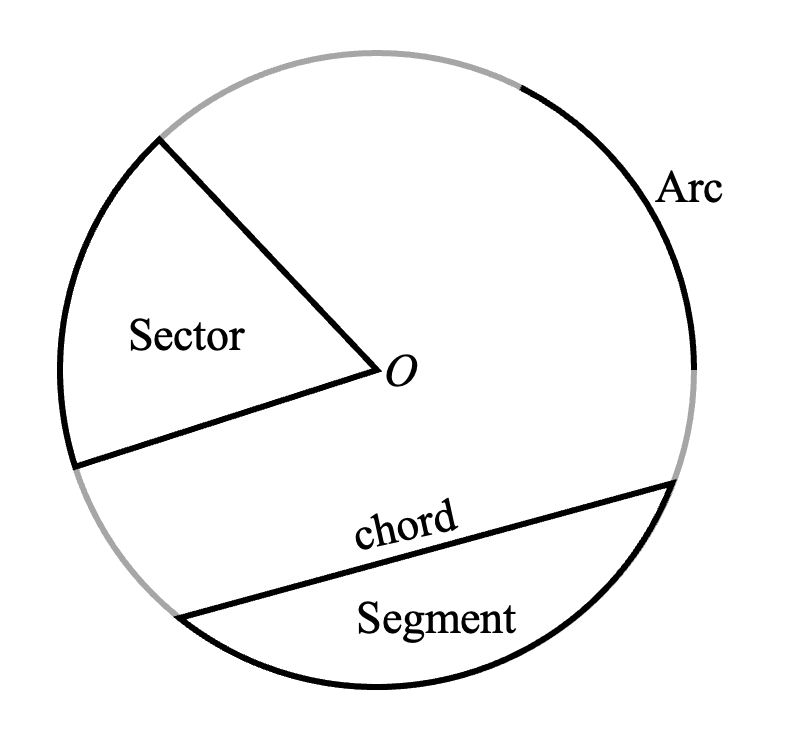
\includegraphics[width=0.5\textwidth]{Fig.18.jpg}
    \end{figure}
    \item If the angle of the arc is $\theta$ (in radian), the length of $\text{arc}(l)=r\cdot\theta$.
    \item The area of a sector: $$\color{red}A=\frac{1}{2}r^2\theta.$$
    \item The area of a segment: $$\color{red}A=\frac{1}{2}r^2(\theta-\sin\theta).$$(Proof: the area of the triangle according to the sine rule is $\frac{1}{2}ab\sin C$)
  \end{itemize}
\end{enumerate}

\subsection{Solution of Triangle}
\begin{enumerate}
  \item Define sine, cosine, and tangent: 
  \begin{myclaim}{ }{}
    \begin{figure}[H]
      \centering
      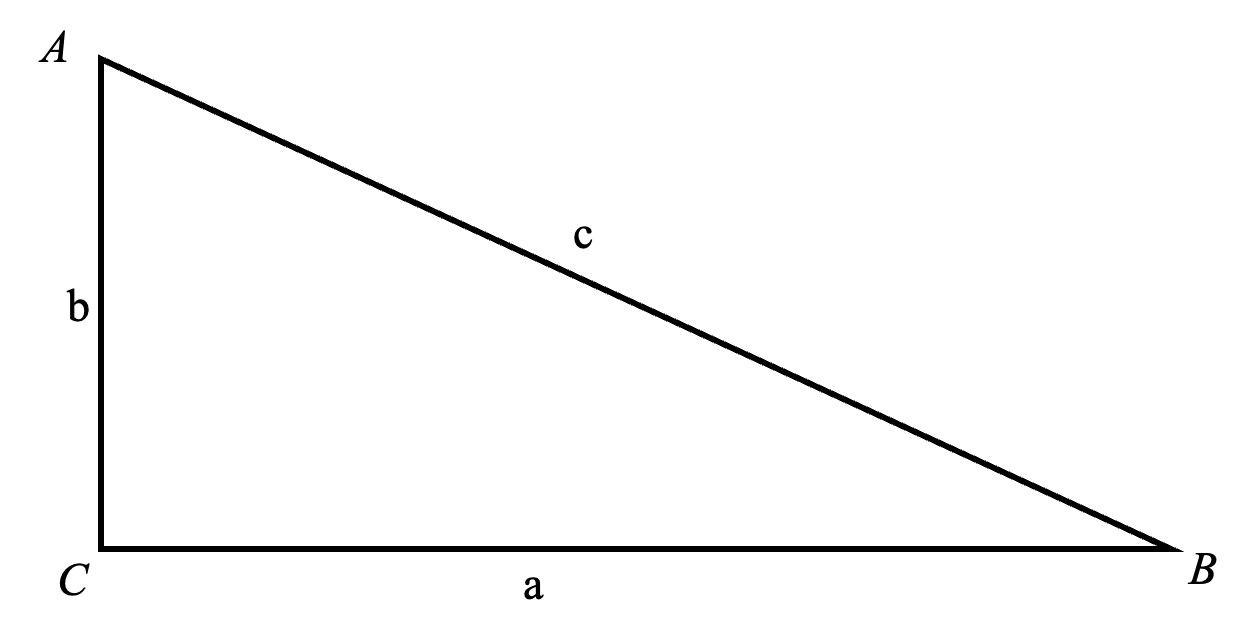
\includegraphics[width=0.5\textwidth]{Fig.19.jpg}
    \end{figure}
    $$\sin A=\frac{a}{c},\ \sin B=\frac{b}{c};$$
    $$\cos A=\frac{b}{c},\ \cos B=\frac{a}{c};$$
    $$\tan A=\frac{a}{b},\ \tan B=\frac{b}{a}.$$
  \end{myclaim}
  \item The Sine Rule: 
  \begin{theorem}{1.2.1 The Sine Rule}{}
    $${\color{red}{\frac{\sin A}{a}=\frac{\sin B}{b}=\frac{\sin C}{c}}}.$$
  \end{theorem}
  \begin{itemize}
    \item The bigger the angle, the longer the side. 
    \item Area of a triangle: $${\color{red}{A=\frac{1}{2}ab\sin C}}.$$
  \end{itemize}
  \item The Consine Rule: 
  \begin{theorem}{1.2.2 The Cosine Rule}{}
    $${\color{red}{b^2+c^2-a^2=2bc\cdot\cos A}};$$
    $${\color{red}{a^2+c^2-b^2=2ac\cdot\cos B}};$$
    $${\color{red}{a^2+b^2-c^2=2ab\cdot\cos C}}.$$
  \end{theorem}
  \item Inverse Trigonometric Functions: 
  \begin{myclaim}{ }{}
    $$\sin^{-1}\theta=\arcsin\theta;$$
    $$\cos^{-1}\theta=\arccos\theta;$$
    $$\tan^{-1}\theta=\arctan\theta.$$
  \end{myclaim}
  \item Ambiguity of Sine Rule: 
  $${\color{red}{\sin\theta=\sin(180^\circ-\theta)\text{ OR }\sin\theta=\sin(\pi-\theta)}}.$$
  \item Angle of Elevation and Depression: 
  \begin{myclaim}{ }{}
    \begin{figure}[H]
      \centering
      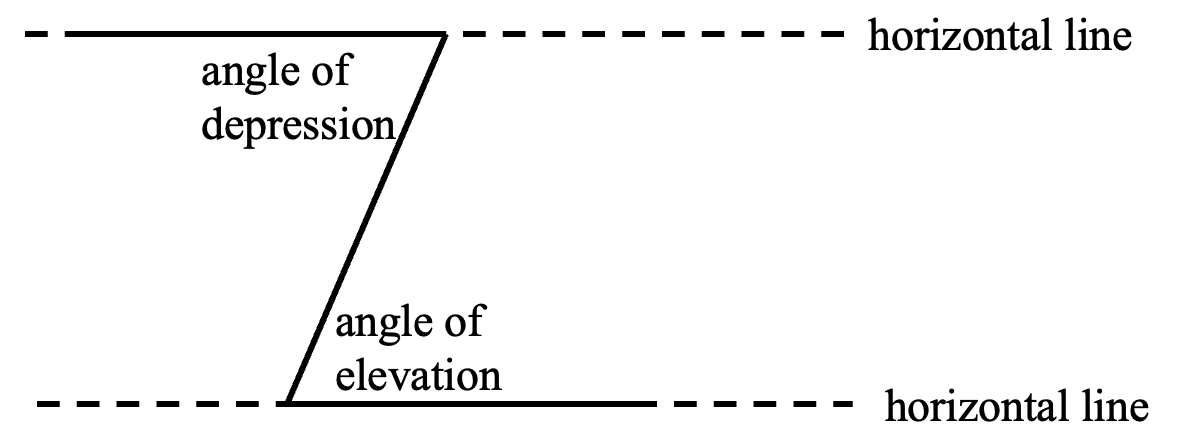
\includegraphics[width=0.8\textwidth]{Fig.20.jpg}
    \end{figure}
    \begin{itemize}
    \item \textbf{\color{red}{Angle of Elevation}} is the angle "up" from horizontal. 
    \item \textbf{\color{red}{Angle of Depression}} is the angle "down" from horizontal. 
    \end{itemize}
  \end{myclaim}
  \item Bearing: 
  \begin{itemize}
    \item Bearing is a way of describing direction. 
    \item All bearings are measured {\color{red}{clockwise}} from the {\color{red}{North}} direction. 
    \begin{figure}[H]
      \centering
      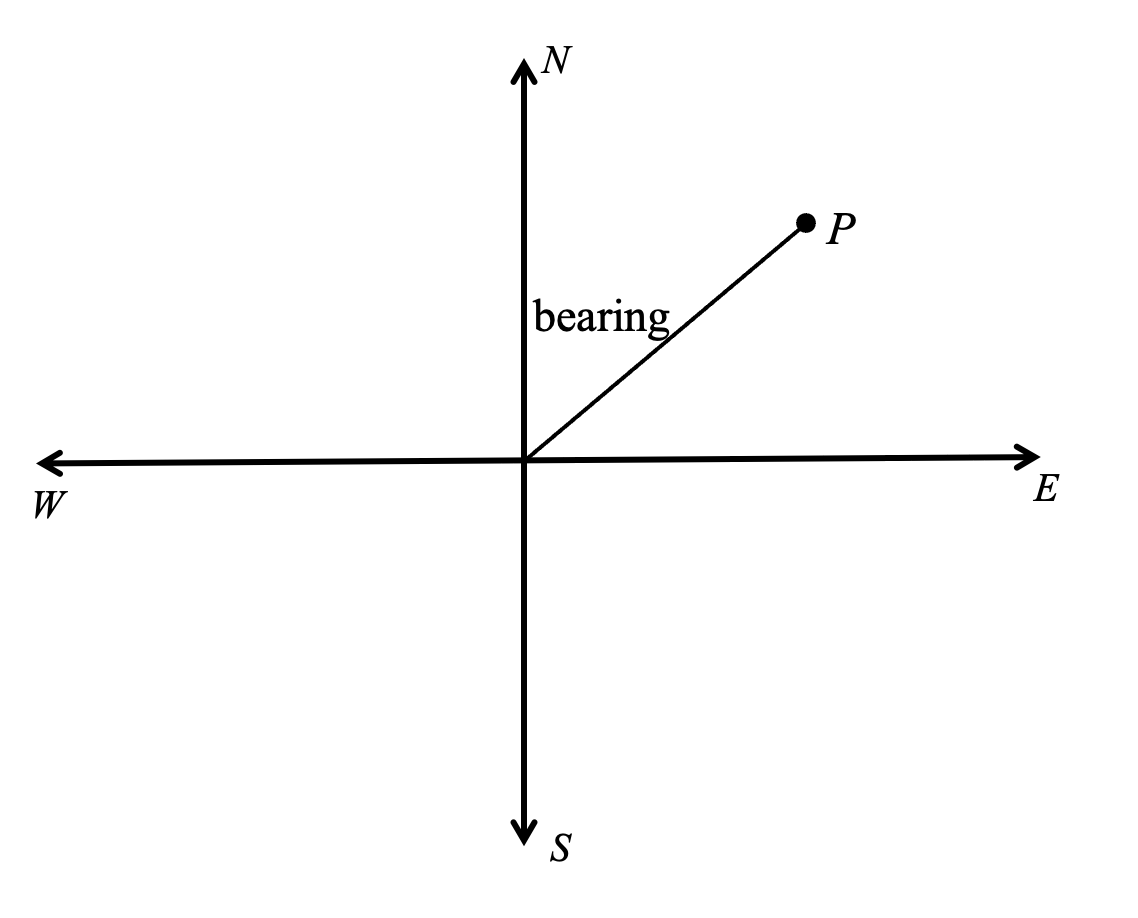
\includegraphics[width=0.5\textwidth]{Fig.21.jpg}
    \end{figure}
  \item Bearing of $A$ from $B$: construct at $B$.\\
  {\color{green}{N.B.: Bearing of $A$ from $B$ is different from bearing of $B$ from $A$.}}
  \end{itemize}
\end{enumerate}

\subsection{Definition of Trigonometric Function}
\begin{enumerate}
  \item Unit Circle: 
  \begin{itemize}
    \item Center at $(0,0)$ with a radius of $1$.
    \begin{figure}[H]
      \centering
      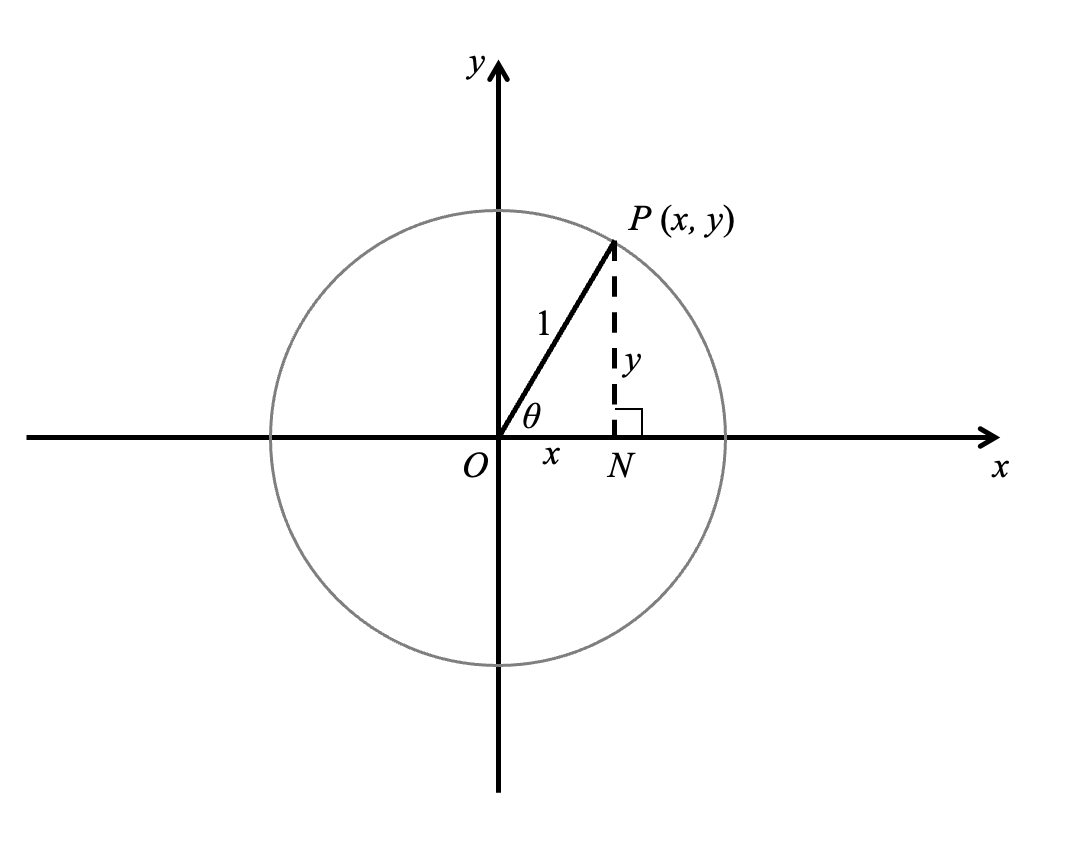
\includegraphics[width=0.5\textwidth]{Fig.22.jpg}
    \end{figure}
    \item If an angel $\theta$ opens in a counterclockwise direction, then $\theta$ is positive. \\
    If an angle $\theta$ opens in a clockwise direction, then $\theta$ is negative. 
    \item In the diagram, $\theta=\theta+2k\pi,\ k\in\Z.$
    \item $$\sin\theta=\frac{PN}{OP}=\frac{y}{1}=y; $$
    $$\cos\theta=\frac{ON}{OP}=\frac{x}{1}=x; $$
    $$\tan\theta=\frac{PN}{ON}=\frac{y}{x}=\frac{\sin\theta}{\cos\theta}; $$
    \item In $Q_1$ and $Q_2$, $\sin\theta$ will be positive.\\
    In $Q_1$ and $Q_4$, $\cos\theta$ will be positive.\\
    In $Q_1$ and $Q_3$, $\tan\theta$ will be positive.\\
    $\Rightarrow$ CAST: 
    \begin{figure}[H]
      \centering
      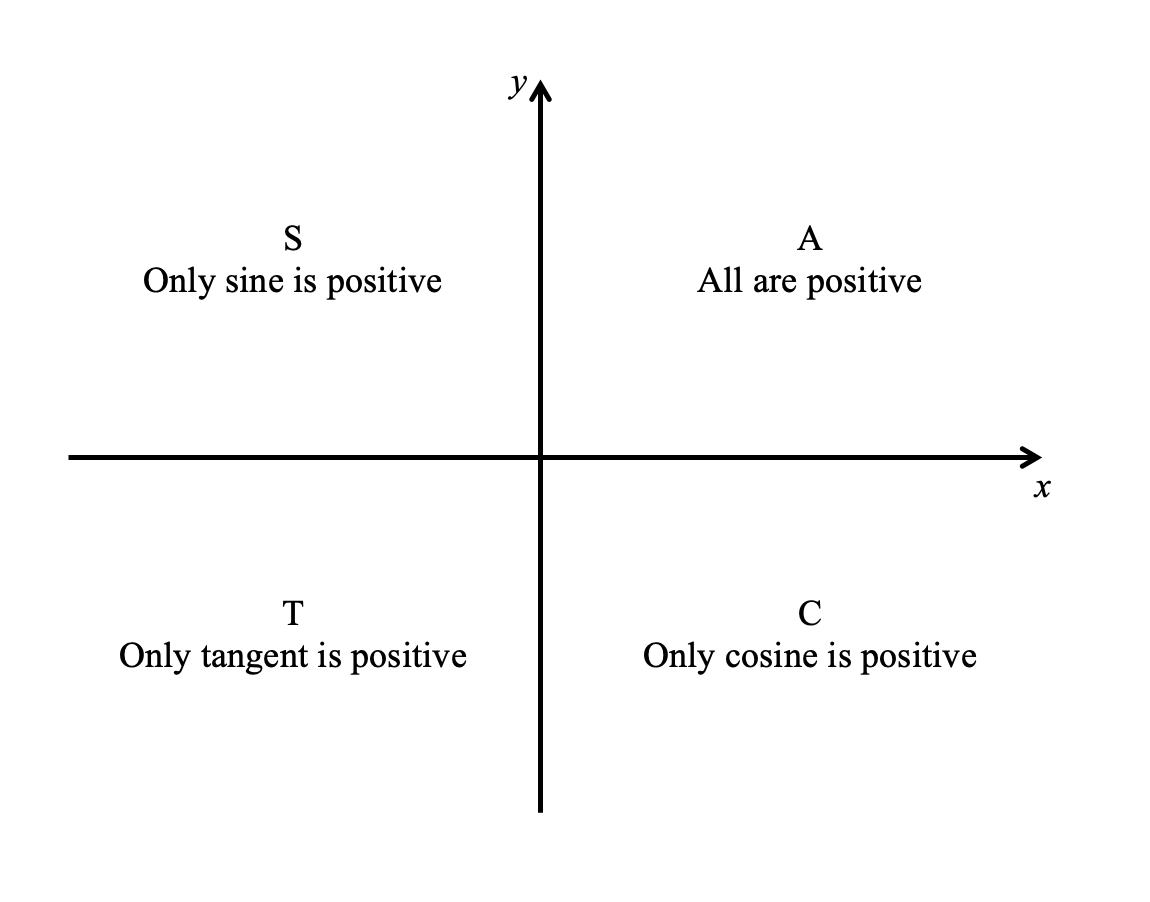
\includegraphics[width=0.5\textwidth]{Fig.23.jpg}
    \end{figure}
  \end{itemize}
  \item Special Angles: 
  \begin{multicols}{2}
    $$\sin0^\circ=0=\cos90^\circ$$
    $$\sin30^\circ=\frac{1}{2}=\cos60^\circ$$
    $$\sin45^\circ=\frac{\sqrt{2}}{2}=\cos45^\circ$$
    $$\sin60^\circ=\frac{\sqrt{3}}{2}=\cos30^\circ$$
    $$\sin90^\circ=1=\cos0^\circ$$
    $$\tan0^\circ=\frac{\sin0^\circ}{\cos0^\circ}=0$$
    $$\tan30^\circ=\frac{\sin30^\circ}{\cos30^\circ}=\frac{\sqrt{3}}{3}$$
    $$\tan45^\circ=\frac{\sin45^\circ}{\cos45^\circ}=1$$
    $$\tan60^\circ=\frac{\sin60^\circ}{\cos60^\circ}=\sqrt{3}$$
    $$\tan90^\circ=\frac{\sin90^\circ}{\cos90^\circ}=\infty$$
  \end{multicols}
  \item Relative Acute Angles (RAA): 
  \begin{itemize}
    \item Acute angle is the angle with $x$-axis.
    \item The absolute value of angles have the same acute angle is the same. 
    \begin{example}{1.3.1}{}
      \begin{enumerate}
        \item $30^\circ,\ 150^\circ,\ 210^\circ,\ 330^\circ$ have the same acute angle. \\
        $\therefore \left|\sin30^\circ\right|=\left|\sin150^\circ\right|=\left|\sin210^\circ\right|=\left|\sin330^\circ\right|.$
        \item $$\tan220^\circ=\tan40^\circ;\ \cos215^\circ=-\cos35^\circ$$
        \begin{figure}[H]
          \centering
          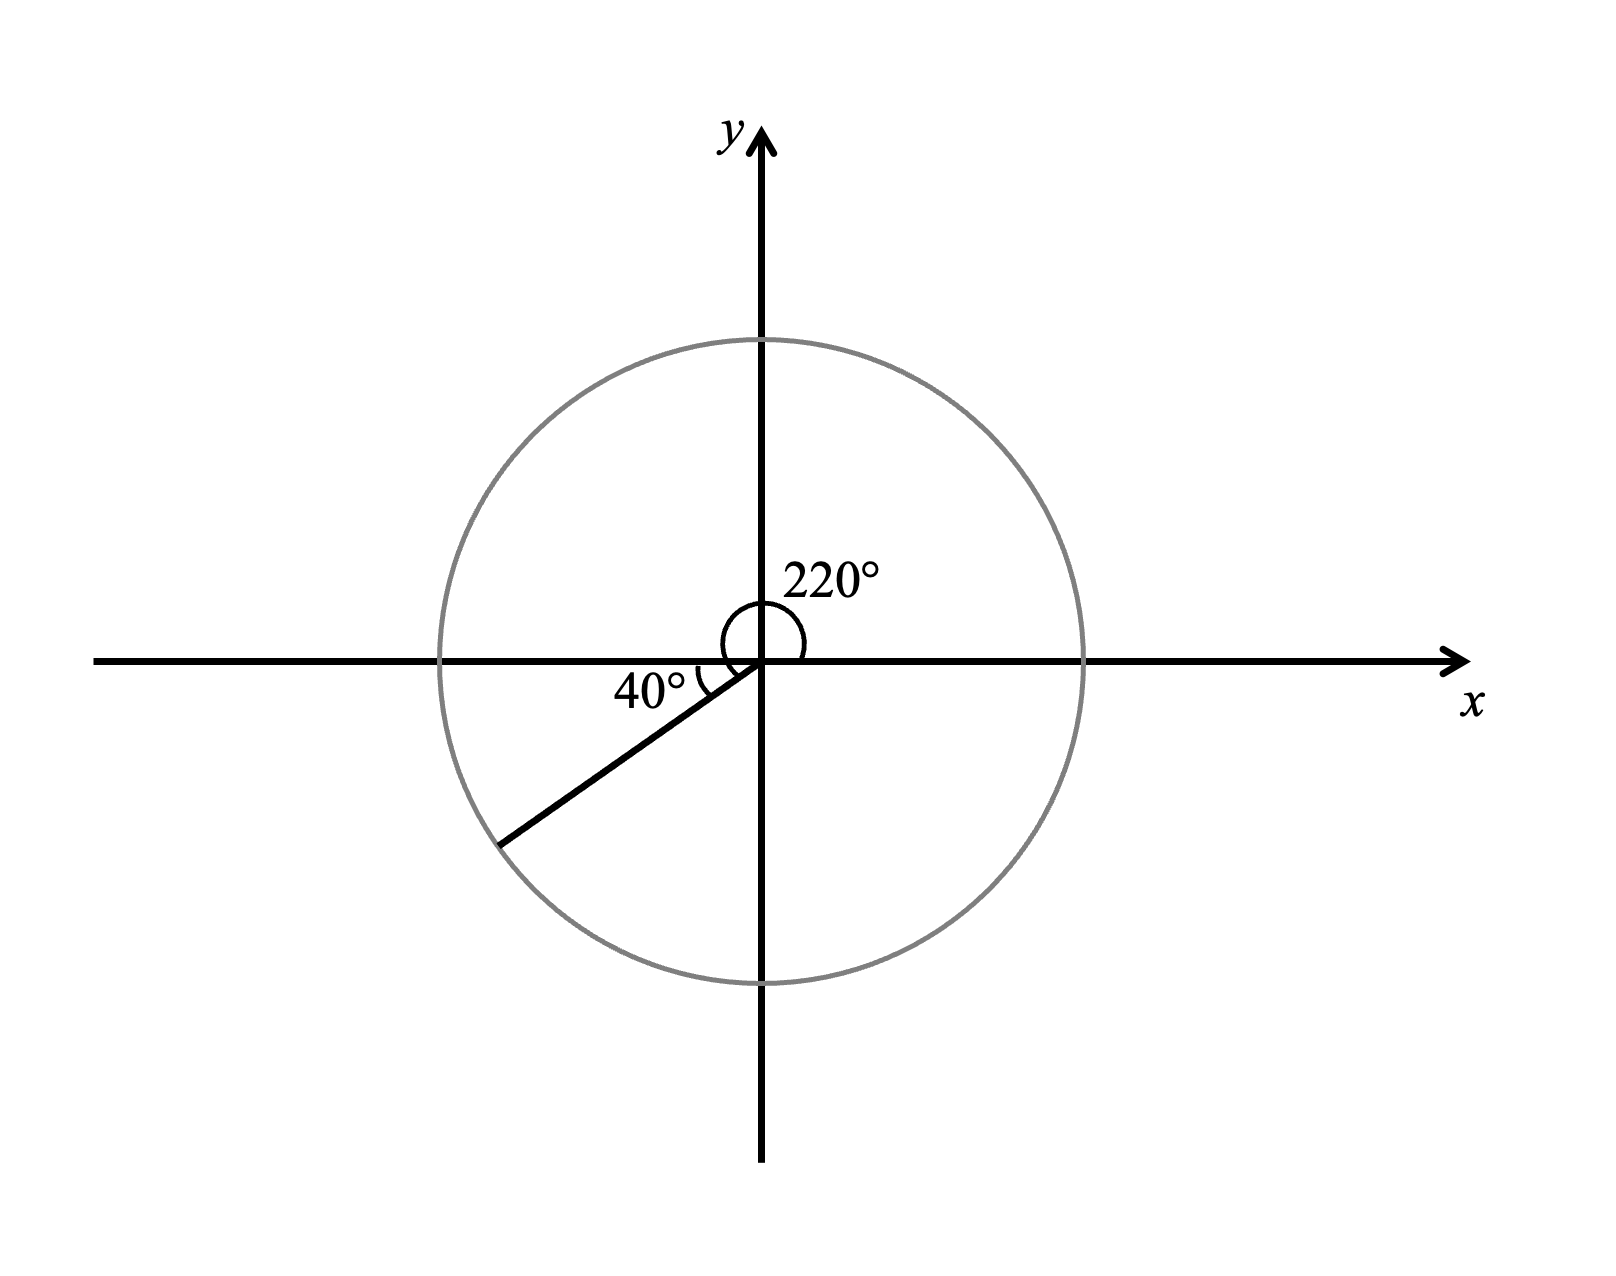
\includegraphics[width=0.5\textwidth]{Fig.24.jpg}
        \end{figure}
      \end{enumerate}
    \end{example}
  \end{itemize}
\end{enumerate}

\subsection{Trigonometric Identity}
\begin{enumerate}
  \item Pythagorean's Identity: 
  $${\color{red}{\sin^2\theta+\cos^2\theta\equiv1}}.$$
  \begin{proof}{1.4.1}{}
    $$\begin{aligned}
      a^2+b^2=c^2&\Rightarrow\frac{a^2}{c^2}+\frac{b^2}{c^2}=1\\
      &\Rightarrow\sin^2\theta+\cos^2\theta=1.
    \end{aligned}$$
  \end{proof}
  \item Definition of Tangent: 
  \begin{itemize}
    \item $${\color{red}{\tan\theta=\frac{\sin\theta}{\cos\theta}}};$$
    \item $${\color{red}{\cot\theta=\frac{1}{\tan\theta}}};$$
    \item $${\color{red}{\sec\theta=\frac{1}{\cos\theta}}};$$
    \item $${\color{red}{\csc\theta=\frac{1}{\sin\theta}}}.$$
  \end{itemize}
  \item Extended Pythagorean's Identity: 
  $${\color{red}{\tan^2\theta+1=\sec^2\theta}};$$
  $${\color{red}{\cot^2\theta+1=\csc^2\theta}}.$$
  \begin{proof}{1.4.2}{}
    $$\begin{aligned}
      \sin^2\theta+\cos^2\theta=1\Rightarrow&\frac{\sin^2\theta}{\cos^2\theta}+\frac{\cos^2\theta}{\cos^2\theta}=\frac{1}{\cos^2\theta}\Rightarrow\tan^2+1=\sec^2\theta;\\
      &\frac{\sin^2\theta}{\sin^2\theta}+\frac{\cos^2\theta}{\sin^2\theta}=\frac{1}{\sin^2\theta}\Rightarrow\cot^2\theta+1=csc^2\theta.
    \end{aligned}$$
    {\color{green}{N.B.: a reflex angle is an angle bigger than $180^\circ$, smaller than $360^\circ$.}}
  \end{proof}
  \item Compound Angle Formula: 
  $${\color{red}{\cos(A+B)=\cos{A}\cos{B}-\sin{A}\sin{B}}};$$
  $${\color{red}{\cos(A-B)=\cos{A}\cos{B}+\sin{A}\sin{B}}};$$
  $${\color{red}{\sin(A+B)=\sin{A}\cos{B}+\cos{A}\sin{B}}};$$
  $${\color{red}{\sin(A-B)=\sin{A}\cos{B}-\cos{A}\sin{B}}};$$
  \begin{example}{1.4.1}{}
    \textbf{Find the exact value of $\cos{\frac{\pi}{12}}$.}\\
    \noindent\rule[0.25\baselineskip]{\textwidth}{1pt}
    $$\begin{aligned}
      \cos{\frac{\pi}{12}}&=\cos{\frac{\pi}{4}-\frac{\pi}{6}}\\
      &=\cos{\frac{\pi}{4}}\cos\frac{\pi}{6}+\sin\frac{\pi}{4}\sin\frac{\pi}{6}\\
      &=\frac{\sqrt{2}}{2}\times\frac{\sqrt{3}}{2}+\frac{\sqrt{2}}{2}\times\frac{1}{2}=\frac{\sqrt{6}+\sqrt{2}}{4}.
    \end{aligned}$$
  \end{example}
  $${\color{red}{\tan{(A+B)=\frac{\tan{A}+\tan{B}}{1-\tan{A}\tan{B}}}}}.$$
  \begin{proof}{1.4.3}{}
    $$\begin{aligned}
      \tan{(A+B)}=\frac{\sin{(A+B)}}{\cos{(A+B)}}&=\frac{\sin{A}\cos{B}+\cos{A}\sin{B}}{\cos{A}\cos{B}-\sin{A}\sin{B}}\\
      &=\frac{\frac{\sin{A}\cos{B}}{\cos{A}\cos{B}}+\frac{\cos{A}\sin{B}}{\cos{A}\cos{B}}}{\frac{\cos{A}\cos{B}}{\cos{A}\cos{B}}-\frac{\sin{A}\sin{B}}{\cos{A}\cos{B}}}\\
      &=\frac{\tan{A}+\tan{B}}{1-\tan{A}\tan{B}}.
    \end{aligned}$$
  \end{proof}
  $${\color{red}{\tan{(A-B)}=\frac{\tan{A}-\tan{B}}{1+\tan{A}\tan{B}}}}.$$
  \item In the linear function $y=mx+b$, ${\color{red}{m=\tan\theta}}$, where $\theta$ is the angle between the line and the positive $x$-axis. 
  \item Double Angle Formula: 
  $${\color{red}{\cos{(2\theta)}=\cos^2\theta-\sin^2\theta=2\cos^2\theta-1=1-2\sin^2\theta}};$$
  $${\color{red}{\sin{(2\theta)}=2\sin\theta\cos\theta}};$$
  $${\color{red}{\tan{(2\theta)}=\frac{2\tan\theta}{1-\tan^2\theta}}}.$$
  \item Proving Identities. 
\end{enumerate}

\subsection{Trigonometric Functions and Transformation}
\begin{enumerate}
  \item Sine: Odd function: $\sin{(-x)}=-\sin{x}$.
  \begin{figure}[H]
    \centering
    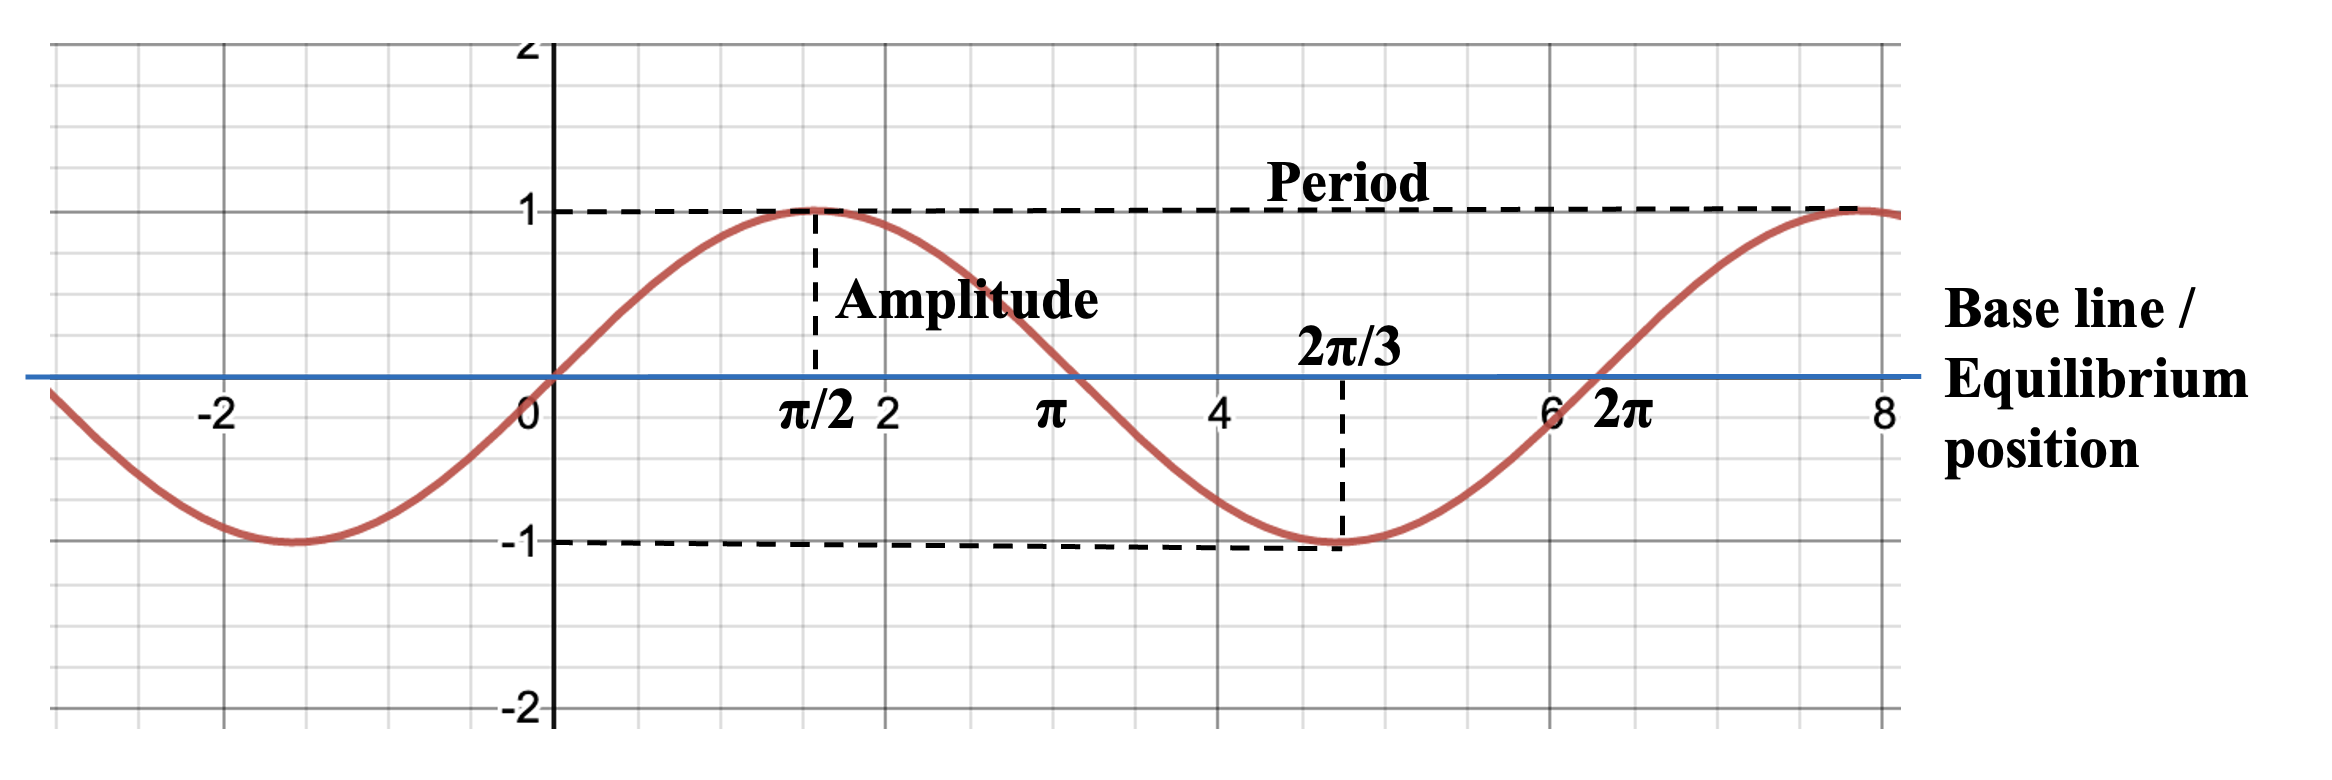
\includegraphics[width=0.9\textwidth]{Fig.25.jpg}
  \end{figure}
  $$\text{T(Period)}=2\pi;$$
  $$\text{Base line}=0;$$
  $$\text{Amplitude}=\left|\frac{y_{\text{max}}-y_{\text{min}}}{2}\right|=1;$$
  $$\text{Range: }\sin{x}\in\left[-1,\ 1\right];$$
  $$\text{Domain: }x\in\R.$$
  \item Cosine: Even function: $\cos{(-x)}=\cos{x}$.
  \begin{figure}[H]
    \centering
    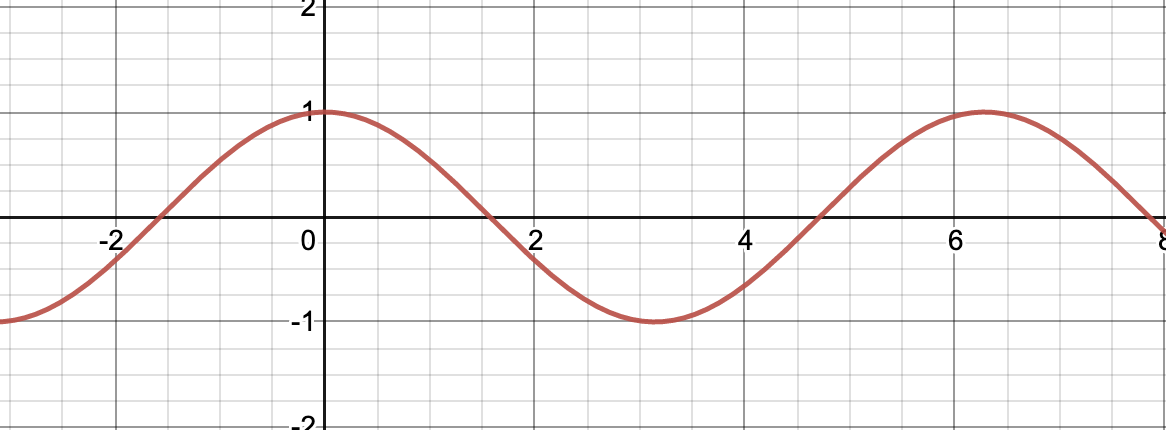
\includegraphics[width=0.85\textwidth]{Fig.26.jpg}
  \end{figure}
  $$\text{T(Period)}=2\pi;$$
  $$\text{Base line}=0;$$
  $$\text{Amplitude}=\left|\frac{y_{\text{max}}-y_{\text{min}}}{2}\right|=1;$$
  $$\text{Range: }\cos{x}\in\left[-1,\ 1\right];$$
  $$\text{Domain: }x\in\R.$$
  \item Tangent: 
  \begin{figure}[H]
    \centering
    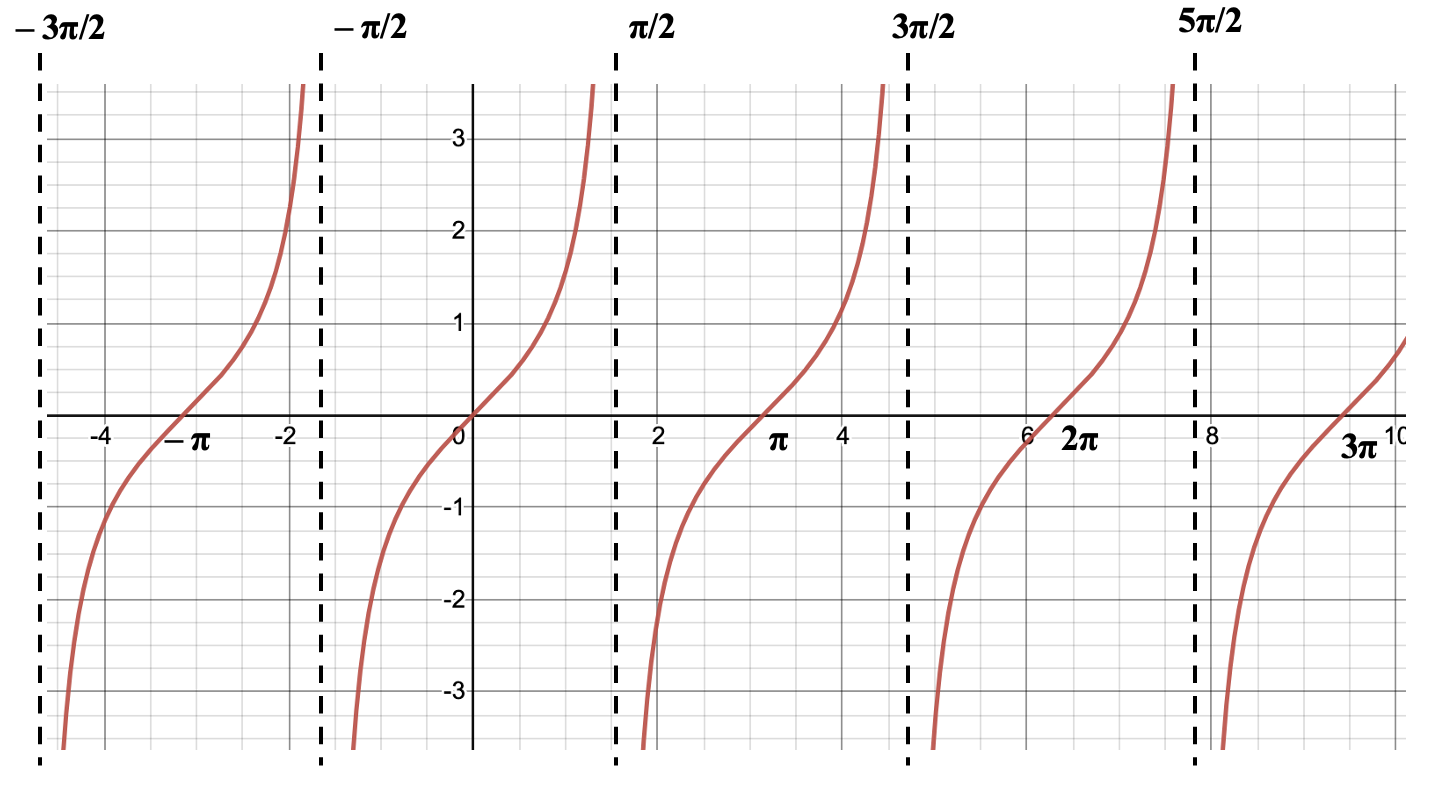
\includegraphics[width=0.9\textwidth]{Fig.27.jpg}
  \end{figure}
  $$\text{T(Period)}=\pi;$$
  $$\text{No amplitude(A)};$$
  $$\text{V.A.: }x=\frac{\pi}{2}+k\pi,\ k\in\Z;$$
  $$\text{Range: }\tan{x}\in\R;$$
  $$\text{Domain: }x\neq\frac{\pi}{2}+k\pi,\ k\in\Z.$$
  \item Transformation of Sine and Cosine: 
  $${\color{red}{y=A\sin{\left(\omega(x-\varphi)\right)}+h}}.$$
  \begin{itemize}
      \item Horizontal stretch with the scale factor of $\frac{1}{\omega}.\ \Rightarrow\ {\color{red}{\text{changes }T=\frac{\pi}{\omega}}}.$
      \item Horizontal translate to the right $\varphi$ units. $\Rightarrow$ {\color{red}{changes the initial point to $(\varphi, 0)$}}.
      \item Vertical stretch with a scale factor of $A$. $\Rightarrow$ {\color{red}{changes the amplitude$=|A|$}}. 
      \item Vertical translation of $h$ units upwards. $\Rightarrow$ {\color{red}{changes the equilibrium position $y=h$}}.
      \item Range of $y=A\sin{\left(\omega(x-\varphi)\right)}+h$: $y\in\left[h-A, h+A\right]$.
  \end{itemize}
  $${\color{red}{y=A\cos\left(\omega(x-\varphi)\right)+h}}.$$
  \begin{itemize}
    \item Horizontal stretch with the scale factor of $\frac{1}{\omega}.\ \Rightarrow\ {\color{red}{\text{changes }T=\frac{\pi}{\omega}}}.$
    \item Horizontal translate to the right $\varphi$ units. $\Rightarrow$ {\color{red}{changes the initial point to $(\varphi, 1)$}}.
    \item Vertical stretch with a scale factor of $A$. $\Rightarrow$ {\color{red}{changes the amplitude$=|A|$, initial point $(\varphi, A)$}}. 
    \item Vertical translation of $h$ units upwards. $\Rightarrow$ {\color{red}{changes the equilibrium position $y=h$, initial point $(\varphi, A+h)$}}.
  \end{itemize}
  \item Cotangent: 
  \begin{figure}[H]
    \centering
    \includegraphics[width=0.85\textwidth]{Fig.28.jpg}
  \end{figure}
  $$\text{V.A.: }x=k\pi$$
  $$\text{Period: }\pi$$
  $$\text{Pass through}\left(\frac{\pi}{2}+k\pi, 0\right)$$
  \item Cosecant: 
  \begin{figure}[H]
    \centering
    \includegraphics[width=0.85\textwidth]{Fig.29.jpg}
  \end{figure}
  $$\text{Domain: }x\neq k\pi$$
  $$\text{Range: }y\in\left.\right]-\infty,-1\left[\right.\cup\left.\right]1,+\infty\left[\right.$$
  \item Secant: 
  \begin{figure}[H]
    \centering
    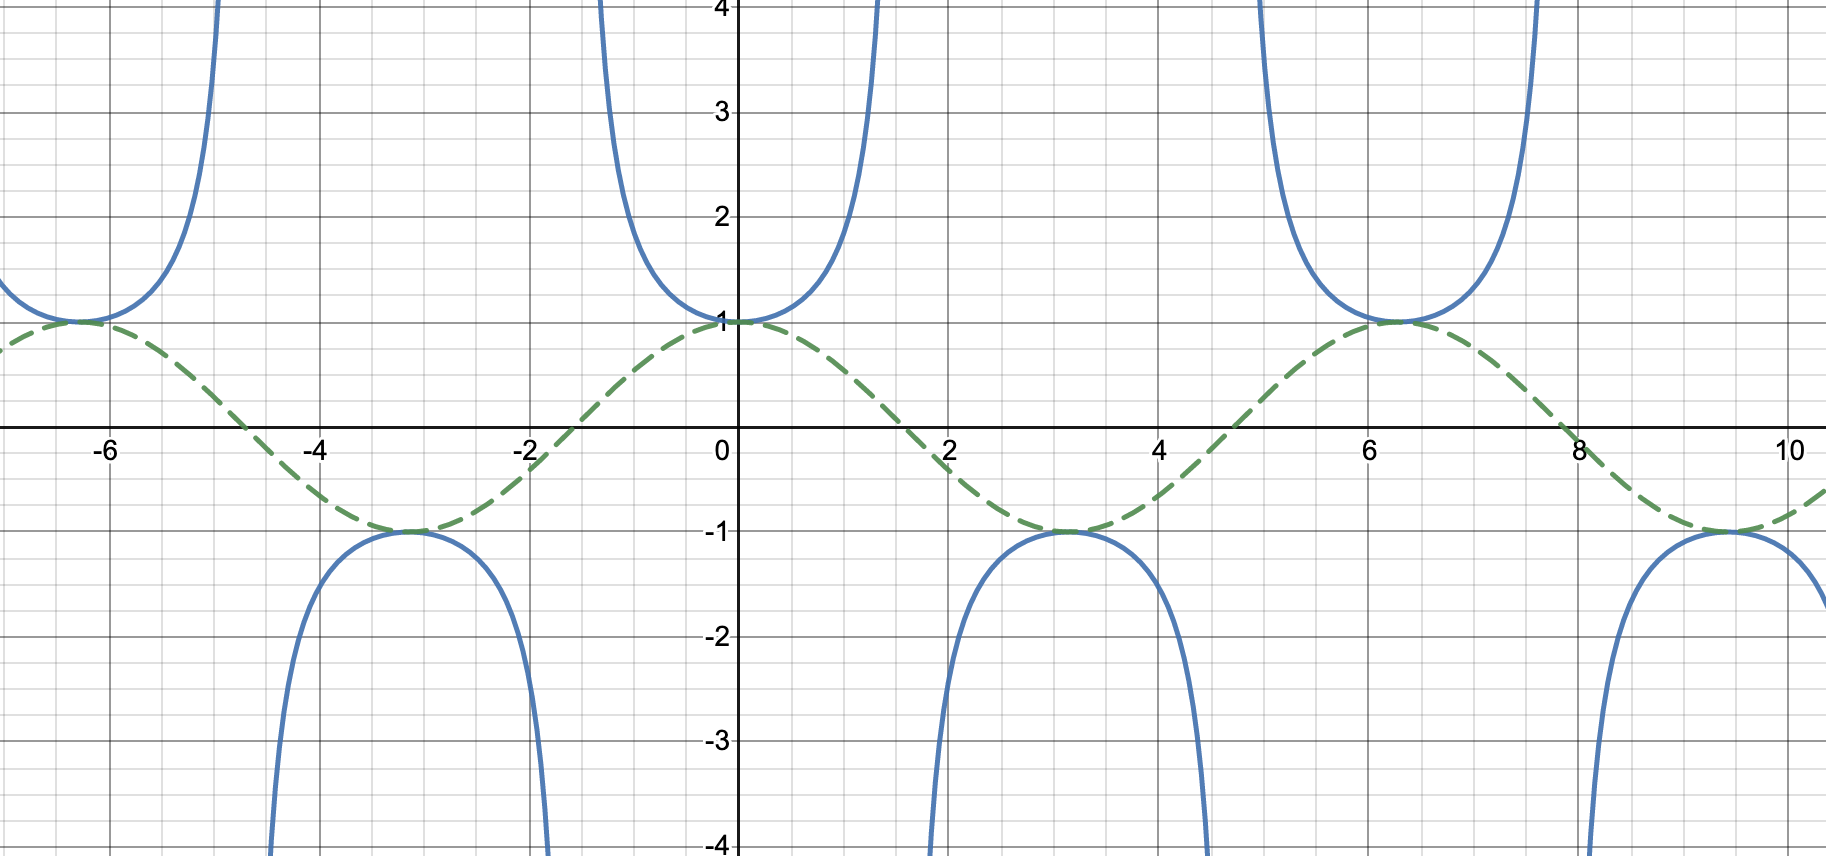
\includegraphics[width=0.85\textwidth]{Fig.30.jpg}
  \end{figure}
  $$\text{Domain: }x\neq\frac{\pi}{2}+k\pi$$
  $$\text{Range: }y\in\left.\right]-\infty,-1\left[\right.\cup\left.\right]1,+\infty\left[\right.$$
  \item When drawing the graph of $sec{x}$ and $\csc{x}$, draw $cos{x}$ and $\sin{x}$ first. 
  \item Conversion between sine and cosine: 
  \begin{itemize}
    \item $$\sin{\left(\frac{\pi}{2}-x\right)}=\cos{x}$$
    \item $$\cos{\left(\frac{\pi}{2}-x\right)}=\sin{x}$$
    \item $$\cos{\left(\frac{\pi}{2}+x\right)}=\cos\left[\pi-\left(\frac{\pi}{2}-x\right)\right]=-\cos{\left(\frac{\pi}{2}-x\right)}=-\sin{x}$$
    \item $$\sin{\left(\frac{\pi}{2}+x\right)}=\sin\left[\pi-\left(\frac{\pi}{2}-x\right)\right]=\sin{\left(\frac{\pi}{2}-x\right)}=\cos{x}$$
  \end{itemize}
\end{enumerate}

\subsection{Solving Trigonometric Functions}
\begin{enumerate}
  \item Solving Trigonometric Functions in Paper 1: 
  \begin{itemize}
    \item Values of sepcial angles
    \item From relative acute angles and CAST rule
    \item Modification of period
    \item Check the solution with domain
  \end{itemize}
  \begin{example}{1.6.1}{}
    \textbf{Solve for $\cos{x}=\frac{\sqrt{3}}{2}$ for $0<x<3\pi$.}\\
    \noindent\rule[0.25\baselineskip]{\textwidth}{1pt}
    $$\text{Consider }x\in[0,2\pi]$$
    $$x=\frac{\pi}{6}, \frac{11\pi}{6}.$$
    $$\text{In the domain of }x\in[0,3\pi],$$
    $$\text{Another solution is }\frac{13\pi}{6}.$$
  \end{example}
  \item Transformed Trigonometric Equations: 
  \begin{example}{1.6.2}{}
    \textbf{Solve $6\sin\left(2\left(x-\frac{\pi}{6}\right)\right)-2=1,\ \frac{\pi}{6}<x<2\pi$.}\\
    \noindent\rule[0.25\baselineskip]{\textwidth}{1pt}
    $$\sin\left(2\left(x-\frac{\pi}{6}\right)\right)=\frac{1}{2}.$$
    $$\text{Let }t=2\left(x-\frac{\pi}{6}\right):$$
  \end{example}
  \begin{example}{1.6.2 - Continued}{}
    $$\because \frac{\pi}{6}<x<2\pi, $$
    $$\therefore 0<2\left(x-\frac{\pi}{6}\right)<\frac{11\pi}{3},\ 0<t<\frac{11\pi}{3}.$$
    $$\sin t=\frac{1}{2}\ \Rightarrow\ t=\frac{\pi}{6},\ \frac{5\pi}{6},\ \frac{13\pi}{6},\ \frac{17\pi}{6};$$
    $$\Rightarrow x=\frac{\pi}{4},\ \frac{7\pi}{12},\ \frac{5\pi}{4},\ \frac{19\pi}{12}.$$
  \end{example}
  \item Solving Trigonometric Functions in Paper 2: 
  \begin{itemize}
    \item Change mode to RADIAN.
    \item Plot the functions. 
    \item Adjust the window. 
    \item Calculate the intersects.
    \item Repeat step 4 if necessary. 
  \end{itemize}
\end{enumerate}

\subsection{Inverse Trigonometric Functions}
\begin{enumerate}
  \item Inverse Trigonometric Function: 
  \begin{itemize}
    \item $$y=\arcsin{x}$$
    \item $$y=\arccos{x}$$
    \item $$y=\arctan{x}$$
    \item $$\text{arcsec}x=\arccos{\left(\frac{1}{x}\right)}$$
    \item $$\text{arccsc}x=\arcsin{\left(\frac{1}{x}\right)}$$
    \item $$\text{arccot}x=\arctan{\left(\frac{1}{x}\right)}$$
  \end{itemize}
  \item One-to-one Function: 
  \begin{itemize}
    \item In order for functions to have the inverse function, it must be so called \textbf{\color{red}{one-to-one}} function (bijection). 
    \item One $x$ value to one (and only one) $y$ value.\\
    One $y$ value to one (and only one) $x$ value. 
  \end{itemize}
  \item Domain and range for $\arcsin{x}$: 
  \begin{itemize}
    \begin{figure}[H]
      \centering
      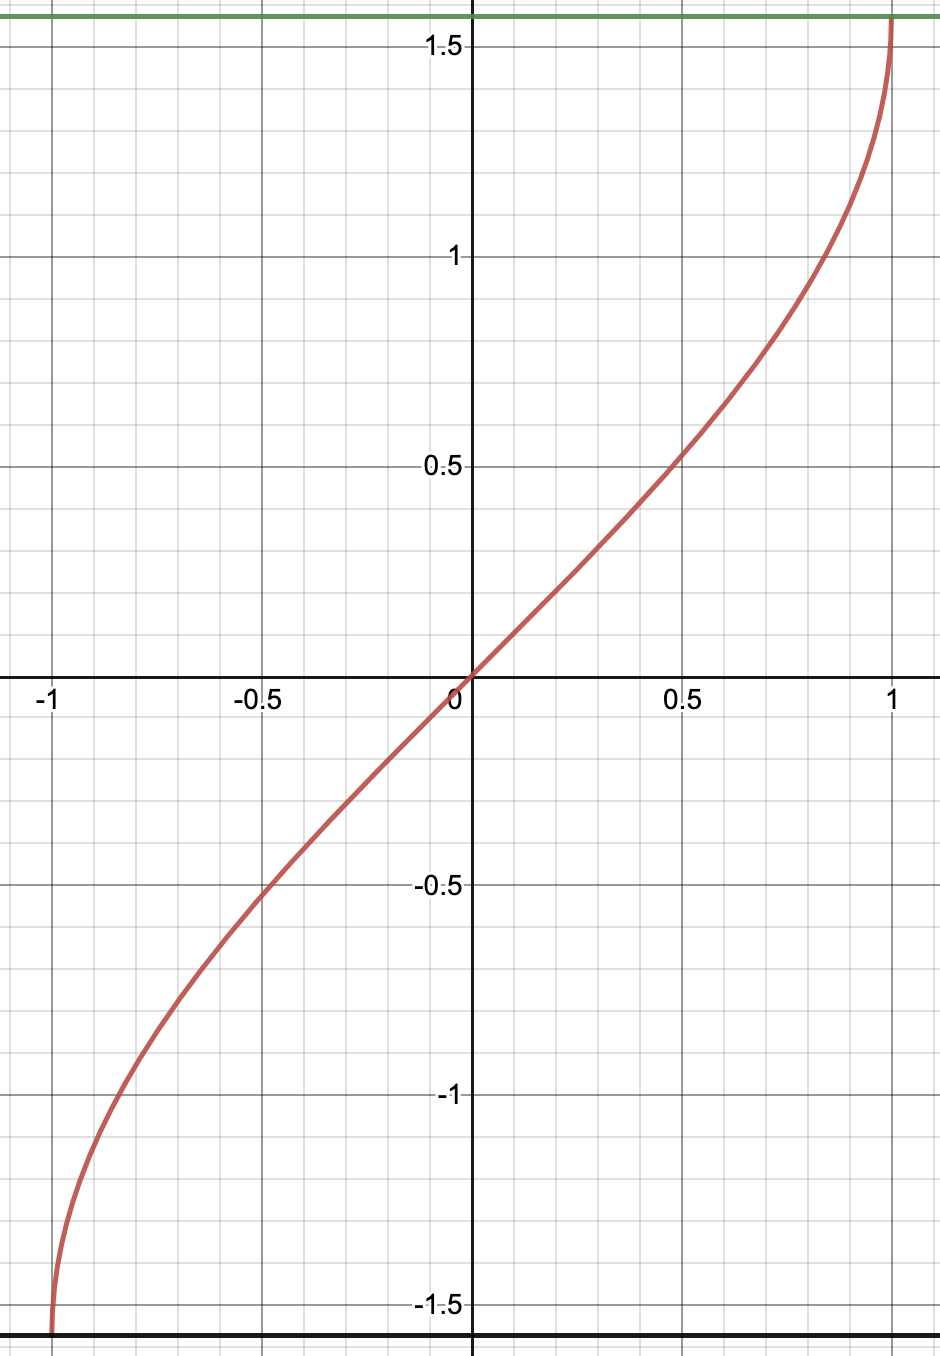
\includegraphics[width=0.45\textwidth]{Fig.31.jpg}
    \end{figure}
    \item Domain: $x\in\left[-1,1\right]$ {\color{green}{(Range $\sin{x}\in\left[-1,1\right]$)}}.
    \item Range: $\arcsin{x}\in\left[-\frac{\pi}{2},\frac{\pi}{2}\right]$ {\color{green}{(Domain $\sin{x}\in\left[-\frac{\pi}{2},\frac{\pi}{2}\right]$)}}.
  \end{itemize}
  \item Domain and range for $\arccos{x}$:
  \begin{itemize}
  \begin{figure}[H]
    \centering
    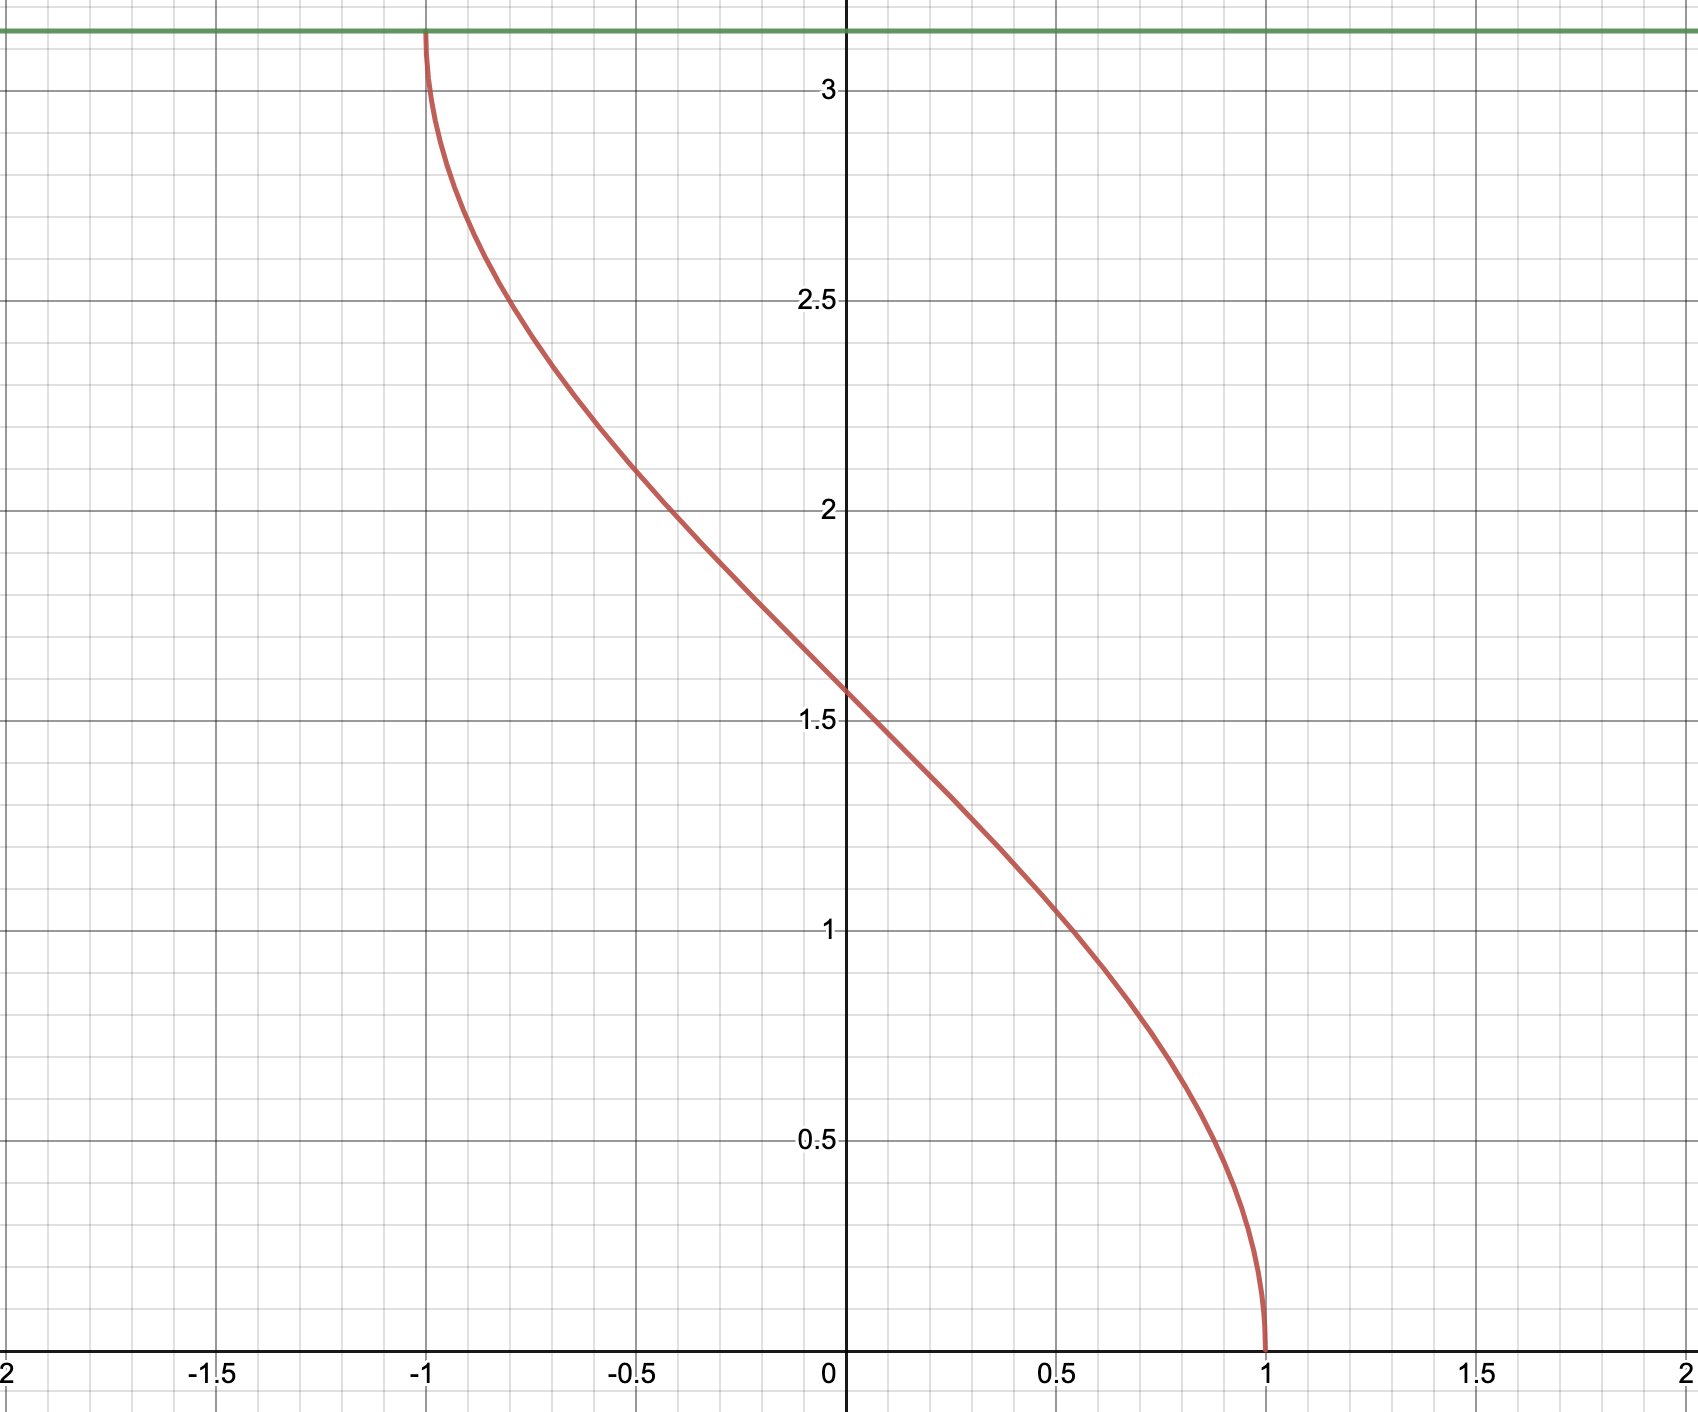
\includegraphics[width=0.6\textwidth]{Fig.32.jpg}
  \end{figure}
  \item Domain: $x\in\left[-1,1\right]$.
  \item Range: $\arccos{x}\in\left[0,\pi\right]$.
  \end{itemize}
  \item Domain and range for $\arctan{x}$: 
  \begin{itemize}
  \begin{figure}[H]
    \centering
    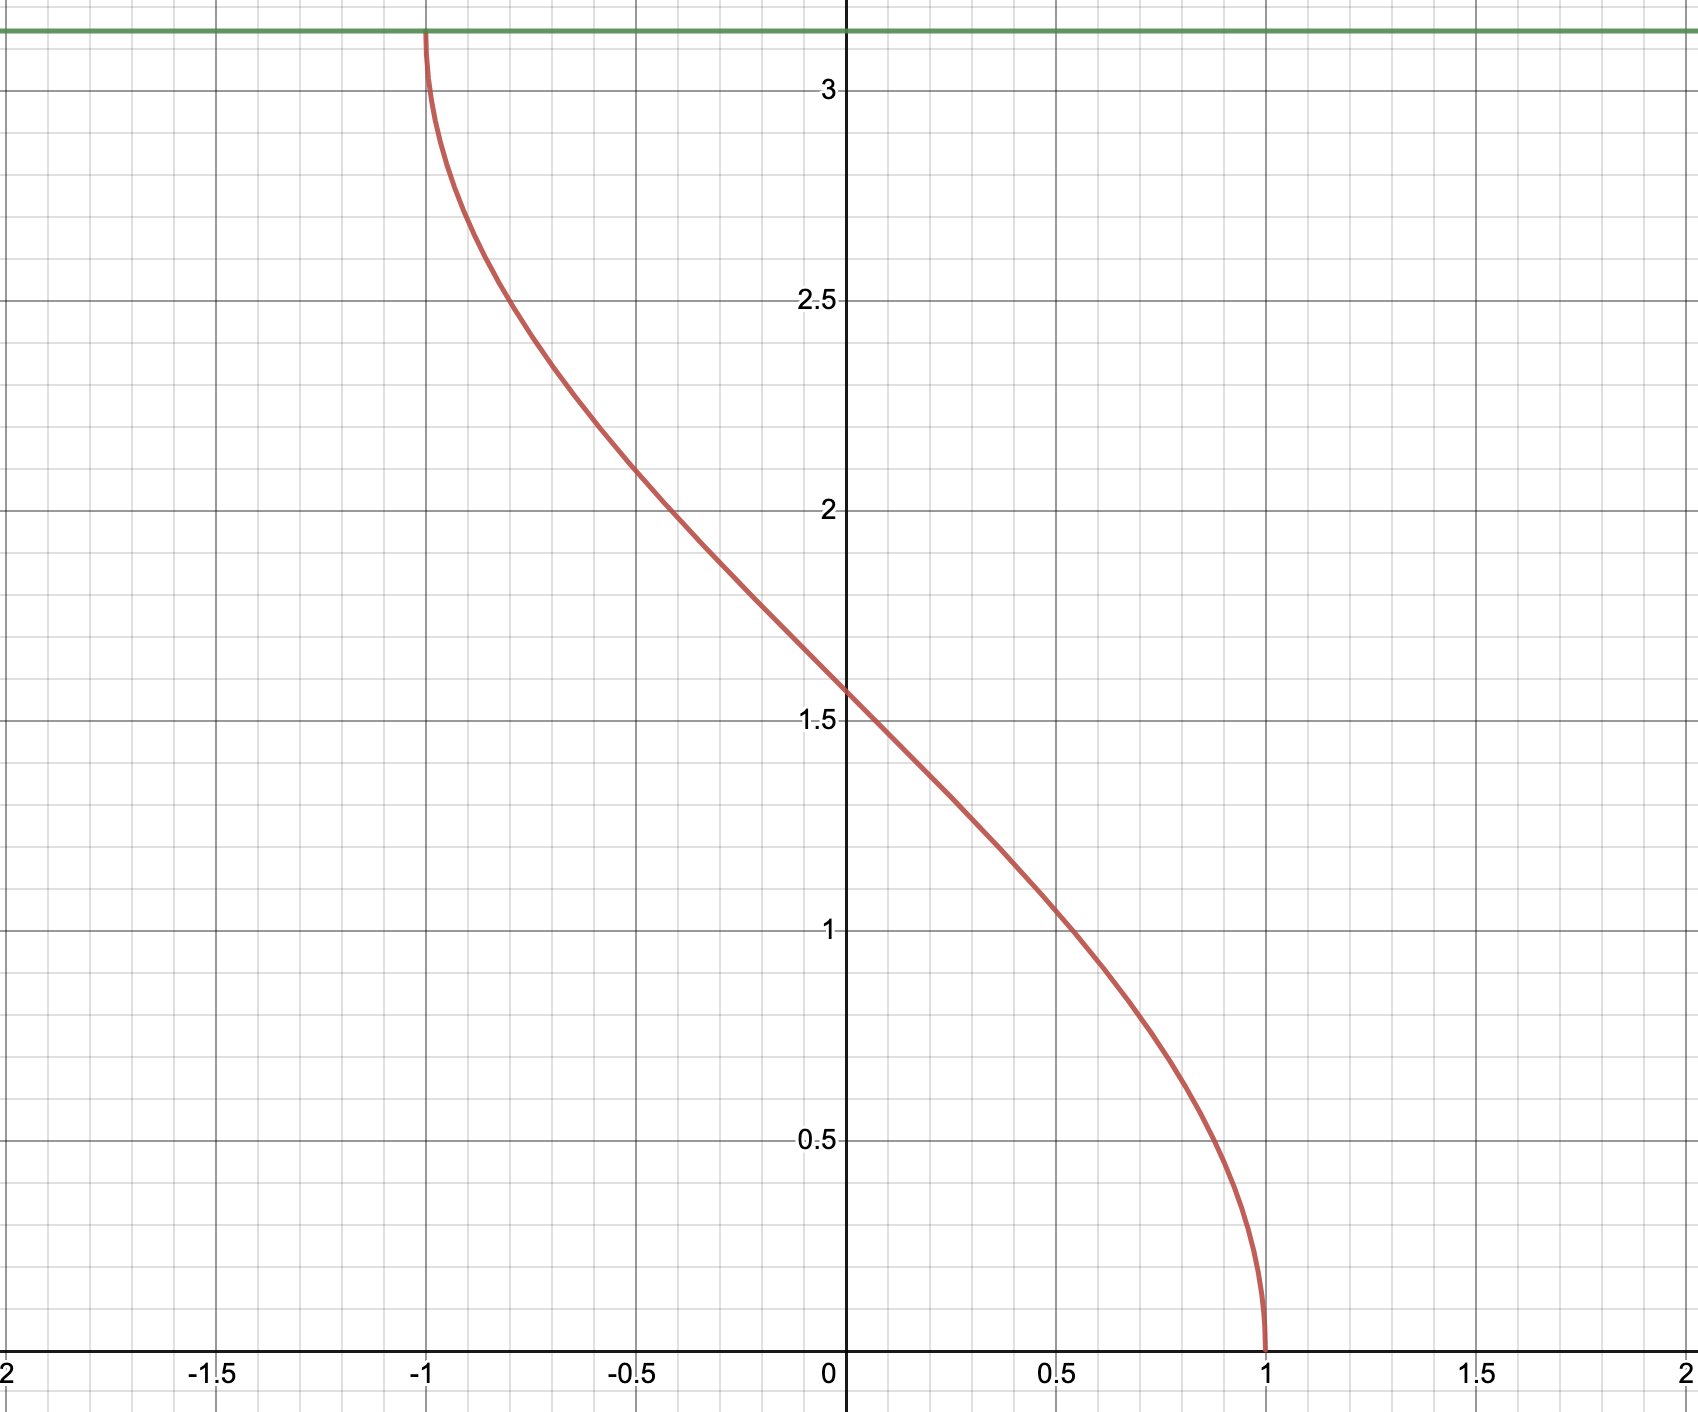
\includegraphics[width=0.6\textwidth]{Fig.32.jpg}
  \end{figure}
  \item Domain: $x\in\R$
  \item Range: $y\in\left.\right]-\frac{\pi}{2},\frac{\pi}{2}\left[\right.$
  \end{itemize}
\end{enumerate}

\newpage
\section{Vectors}
\subsection{Introduction to Vectors}
\begin{enumerate}
  \item Vector: 
  \begin{myclaim}{ }{}
    \\A \textbf{\color{red}{vector}} is a quantity with a direction and magnitude. It is noted as {\color{red}{$\vec{a}$}}.
  \end{myclaim}
  \item Components of a vector: 
  \begin{itemize}
    \item 2-D: 
    \begin{figure}[H]
      \centering
      \includegraphics[width=0.5\textwidth]{Fig.1.jpg}
    \end{figure}
    \begin{example}{2.1.1}{}
      The vector $\vec{a}=\binom{3}{2}$ menas 3 units in the horizontal direction and 2 units in the vertical direction.
    \end{example}
    \item 3D: 
    \begin{figure}[H]
      \centering
      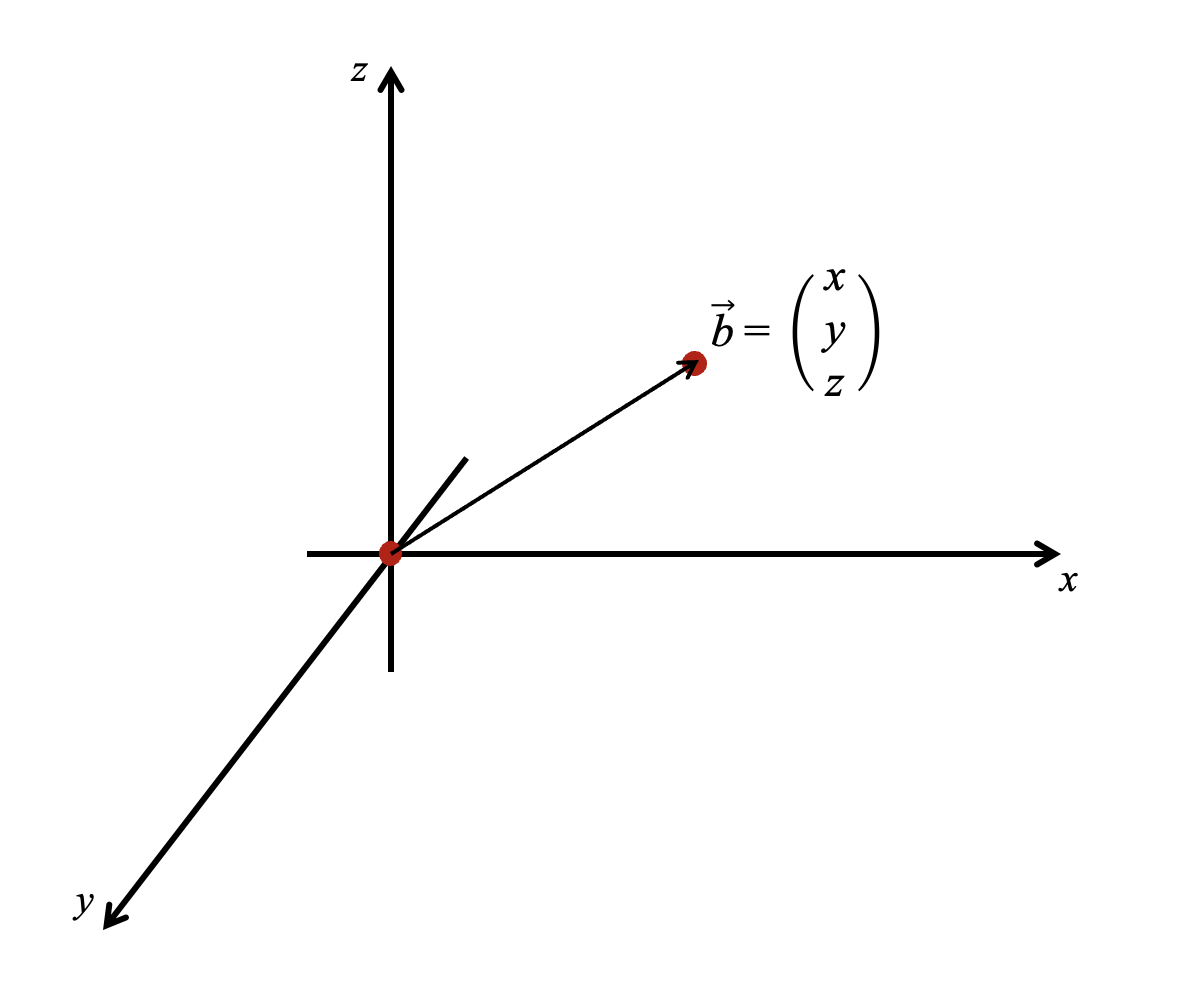
\includegraphics[width=0.5\textwidth]{Fig.2.jpg}
    \end{figure}
  \end{itemize}
  \item \textbf{\color{red}{Magnitude/Modulus}} of vector: 
  \begin{itemize}
    \item 2D: $$\text{For }\vec{a}=\begin{pmatrix}x\\y\end{pmatrix},\ {\color{red}{\left|\vec{a}\right|=\sqrt{x^2+y^2}}}.$$
    \item 3D: $$\text{For }\vec{b}=\begin{pmatrix}x\\y\\z\end{pmatrix},\ {\color{red}{\left|\vec{b}\right|=\sqrt{x^2+y^2+z^2}}}.$$
  \end{itemize}
  \item \textbf{\color{red}{Unit Vector}}: A vector of length 1: 
  \begin{itemize}
    \item $\vec{i}$: unit vector on the $x$-axis.
    \item $\vec{j}$: unit vector on the $y$-axis.
    \item $\vec{k}$: unit vector on the $z$-axis.
    \begin{figure}[H]
      \centering
      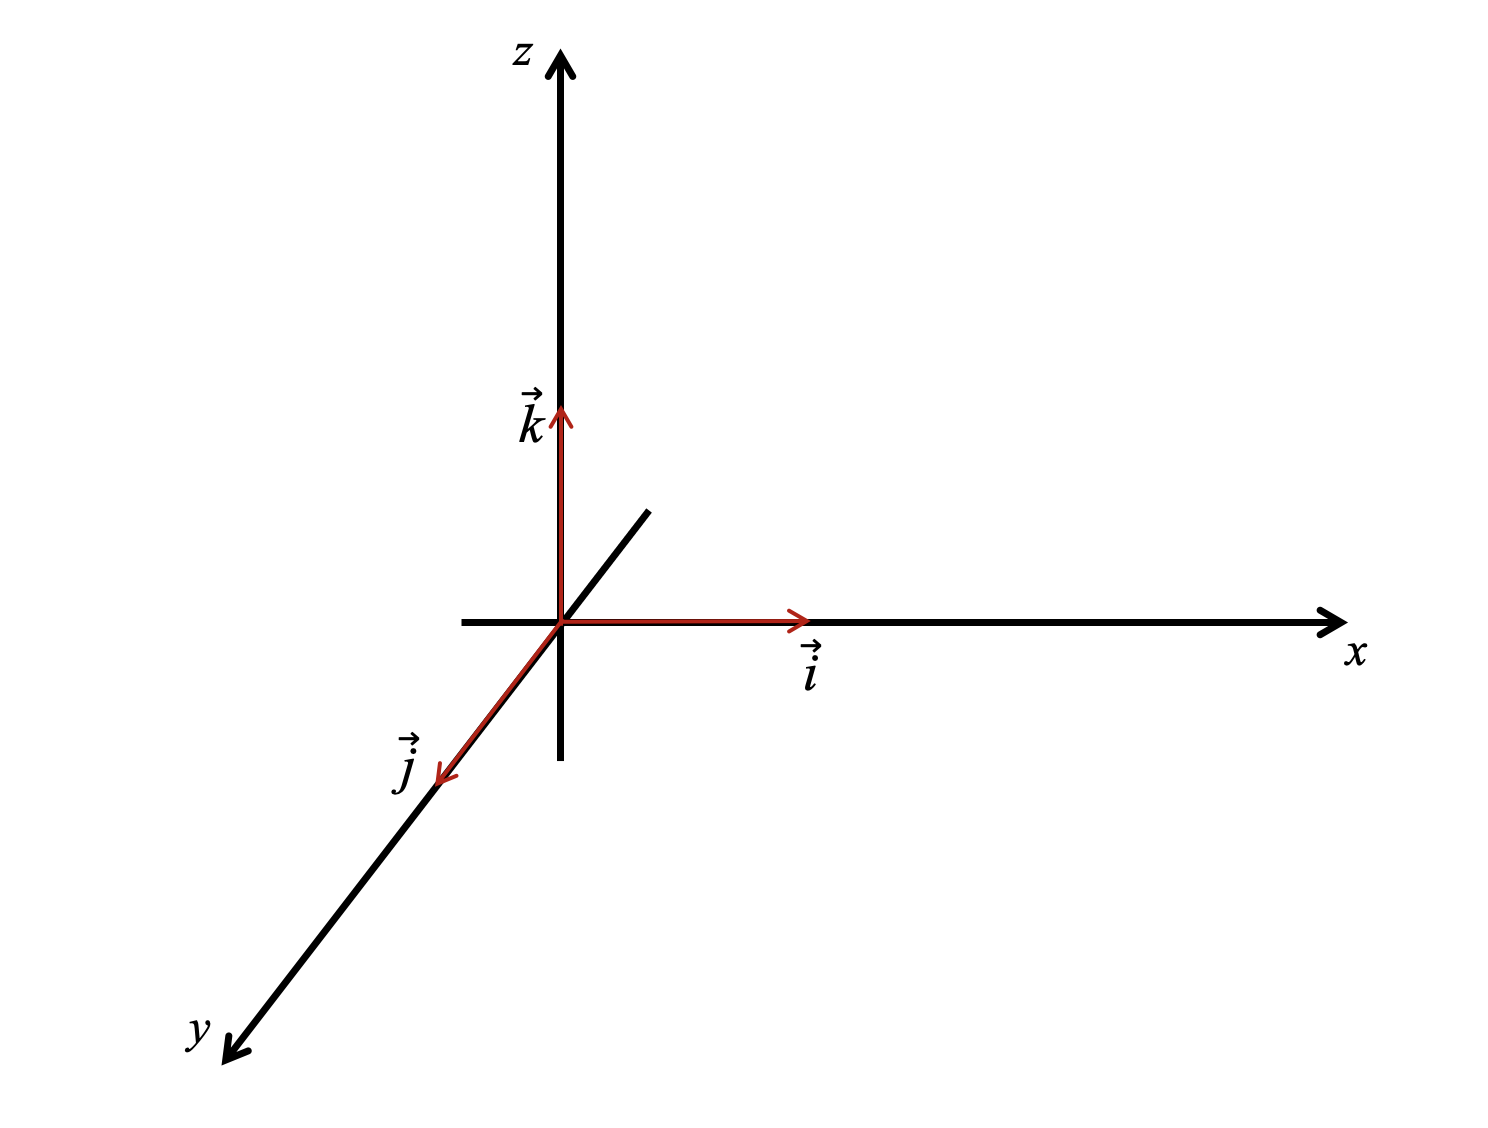
\includegraphics[width=0.5\textwidth]{Fig.3.jpg}
    \end{figure}
  \end{itemize}
  \item Sum of vectors: 
  \begin{itemize}
    \item \textbf{\color{red}{Position vector}}: A vector that has an initial point at the origin. 
    \begin{example}{2.1.2}{}
      $$\vec{a}=\begin{pmatrix}3\\2\end{pmatrix}$$
      $$\vec{a}=3\vec{i}+2\vec{j}.$$
      \begin{figure}[H]
        \centering
        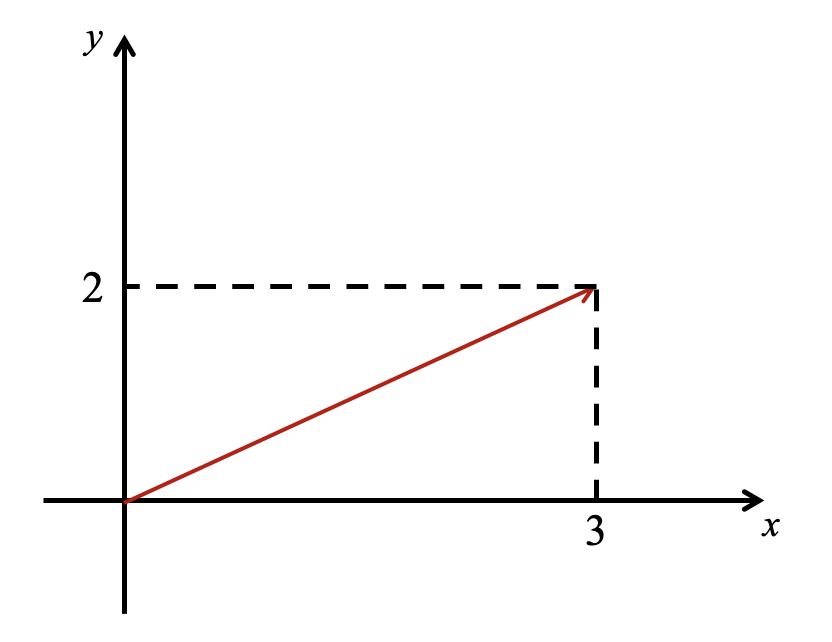
\includegraphics[width=0.5\textwidth]{Fig.4.jpg}
      \end{figure}
    \end{example}
    \item Let $\vec{a}=\begin{pmatrix}x\\y\end{pmatrix}$ and $\vec{b}=\begin{pmatrix}m\\n\end{pmatrix}$
    $${\color{red}{\vec{a}+\vec{b}=\begin{pmatrix}x+m\\y+n\end{pmatrix}}}.$$
  \end{itemize}
  \item Multiplication of vectors by a scalar: \\
  Let $\vec{a}=\begin{pmatrix}x\\y\end{pmatrix}$ and $n$ be a scalar: 
  $${\color{red}{n\vec{a}=n\begin{pmatrix}x\\y\end{pmatrix}=\begin{pmatrix}nx\\ny\end{pmatrix}}}.$$
  {\color{green}{$n\vec{a}$ and $\vec{a}$ are in the same direction $\Rightarrow$ parallel.}}
  \item Subtracting a vector: \\
  Let $\vec{a}=\begin{pmatrix}x\\y\end{pmatrix}$, $\vec{b}=\begin{pmatrix}m\\n\end{pmatrix}$.
  $${\color{red}{\vec{a}-\vec{b}=\begin{pmatrix}x-m\\y-n\end{pmatrix}}}.$$
  \begin{proof}{2.1.1}{}
    $$\begin{aligned}
      -\vec{b}&=(-1)\vec{b}=\begin{pmatrix}-m\\-n\end{pmatrix}\\
      \vec{a}-\vec{b}&=\vec{a}+\left(-\vec{b}\right)=\begin{pmatrix}x-m\\y-n\end{pmatrix}.
    \end{aligned}$$
  \end{proof}
  \item \textbf{\color{red}{Zero vector}}: $\vec{0}$.
  \item \textbf{\color{red}{Collinear points}}: three points, $A$, $B$, and $C$, are said to be collinear if ${\color{red}{\vec{AB}=t\vec{AC}}}$.
  \begin{figure}[H]
    \centering
    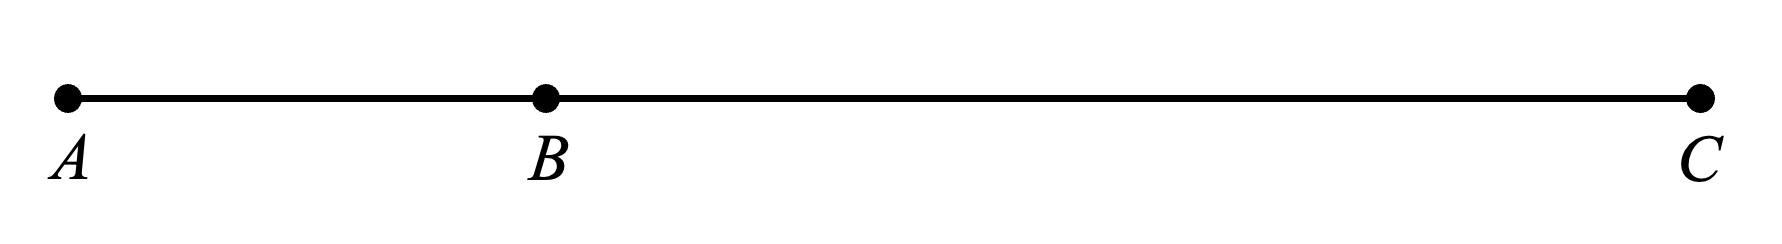
\includegraphics[width=0.5\textwidth]{Fig.5.jpg}
  \end{figure}
  \item Find a unit vector parralel to $\vec{u}=\begin{pmatrix}x\\y\end{pmatrix}.$
  \begin{itemize}
    \item Find the value $\left|\vec{u}\right|.$
    \item Then, the unit vector parralel to $\vec{u}$ is 
    $${\color{red}{\vec{v}=\frac{\vec{u}}{\left|\vec{u}\right|}}}.$$
  \end{itemize}
  \item Vectors and unit circle: 
  \begin{figure}[H]
    \centering
    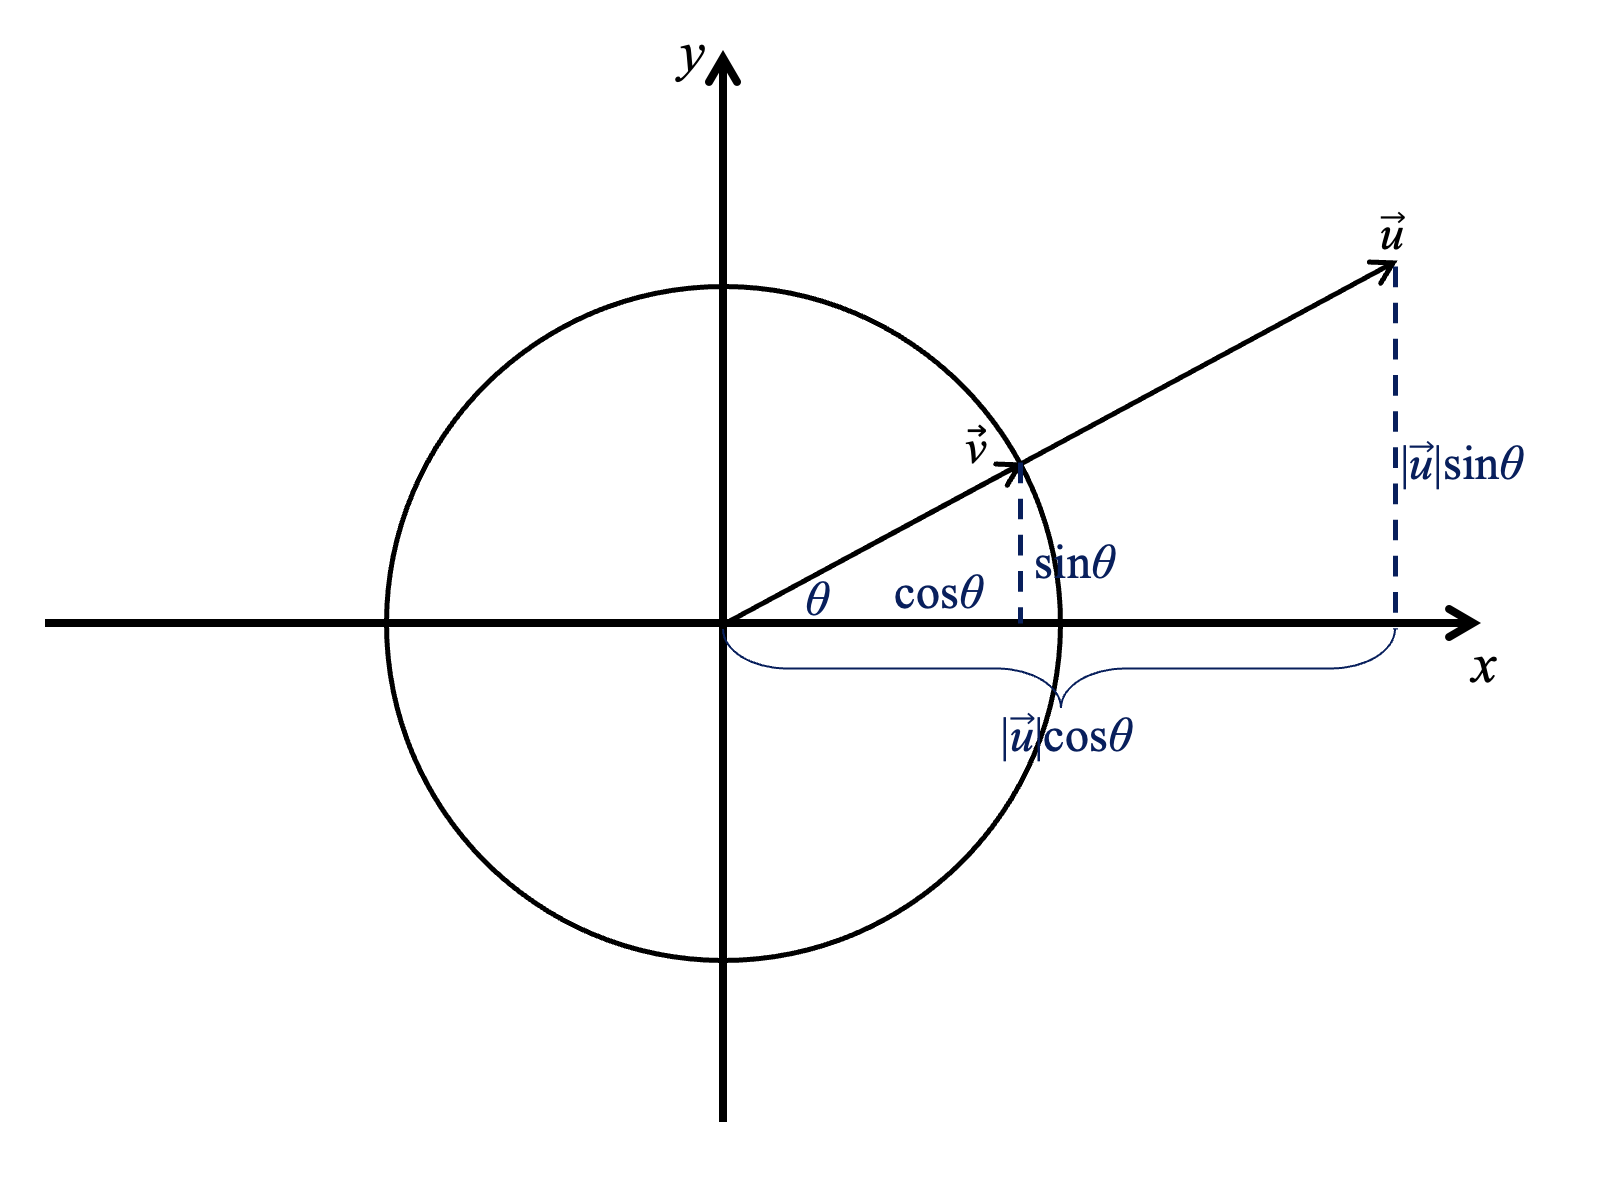
\includegraphics[width=0.5\textwidth]{Fig.6.jpg}
  \end{figure}
  $\theta$ is the angle with the horizontal axis. The unit vector $\vec{v}$, in the same direction as $\vec{u}$ is: 
  $$\vec{v}=\cos\theta\cdot\vec{i}+\sin\theta\cdot\vec{j}\\$$
  $$\begin{aligned}
    \vec{v}=\frac{1}{\left|\vec{u}\right|}\cdot\vec{u}\ \Rightarrow\ \vec{u}=\left|\vec{u}\right|\cdot\vec{v}&=\left|\vec{u}\right|\cos\theta\cdot\vec{i}+\left|\vec{u}\right|\sin\theta\cdot\vec{j}\\
    &=\left|\vec{u}\right|\left(\cos\theta\cdot\vec{i}+\sin\theta\cdot\vec{j}\right).
  \end{aligned}$$
\end{enumerate}

\subsection{Scalar Product and Its Properties}
\begin{enumerate}
  \item The \textbf{\color{red}{scalar product}} of two vectors is a real number (scalar). 
  \begin{itemize}
    \item The algebraic definition: \\
    For $\vec{a}=\begin{pmatrix}a_1\\a_2\end{pmatrix}$ and $\vec{b}=\begin{pmatrix}b_1\\b_2\end{pmatrix}$,
    $${\color{red}{\vec{a}\cdot\vec{b}=\begin{pmatrix}a_1\\a_2\end{pmatrix}\cdot\begin{pmatrix}b_1\\b_2\end{pmatrix}=a_1b_1+a_2b_2}}.$$
    {\color{green}{The scalar product is also called the dot product. }}
    \item The geometric definition: \\
    For $\vec{a}$ and $\vec{b}$,
    $${\color{red}{\vec{a}\cdot\vec{b}=\left|\vec{a}\right|\left|\vec{b}\right|\cos\theta}},\ \theta{\text{is the angle between the two vectors.}}$$
    \begin{proof}{2.2.1}{}
      \begin{figure}[H]
        \centering
        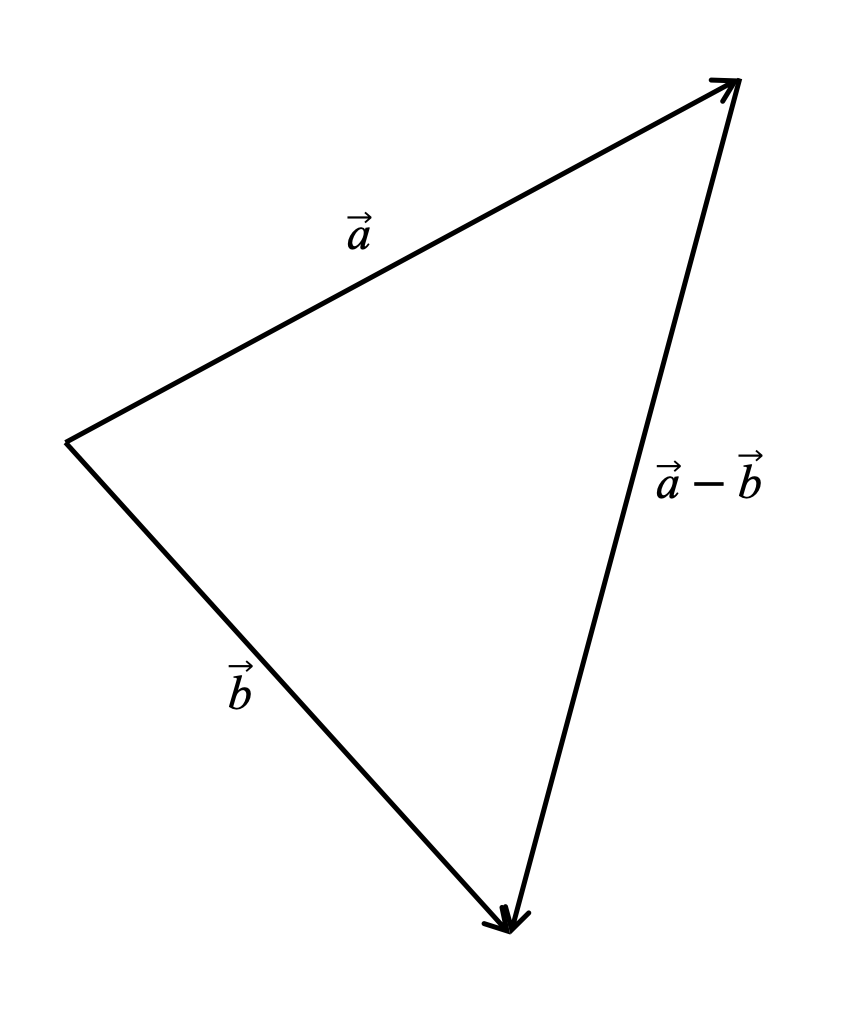
\includegraphics[width=0.5\textwidth]{Fig.7.jpg}
      \end{figure}
      By cosine rule: 
      $$\begin{aligned}
        \left|\vec{b}-\vec{a}\right|^2&=\left|\vec{a}\right|^2+\left|\vec{b}\right|^2-2\left|\vec{a}\right|\left|\vec{b}\right|\cos\theta\\
        \left|\vec{b}\right|^2-2\vec{a}\vec{b}+\left|\vec{a}\right|^2&=\left|\vec{a}\right|^2+\left|\vec{b}\right|^2-2\left|\vec{a}\right|\left|\vec{b}\right|\cos\theta\\
        \therefore \vec{a}\cdot\vec{b}&=\left|\vec{a}\right|\left|\vec{b}\right|\cos\theta.
      \end{aligned}$$
    \end{proof}
    \item Combining the two definitions: 
    $${\color{red}{\cos\theta=\frac{a_1b_1+a_2b_2}{\sqrt{\left(a_1^2+a_2^2\right)\left(b_1^2+b_2^2\right)}}}}.$$
  \end{itemize}
  \item 3-D vectors: $\vec{a}=\begin{pmatrix}a_1\\a_2\\a_3\end{pmatrix}$ and $\vec{b}=\begin{pmatrix}b_1\\b_2\\b_3\end{pmatrix}$: 
  \begin{itemize}
    \item $${\color{red}{\vec{a}\cdot\vec{b}=a_1b_1+a_2b_2+a_3b_3}}.$$
    \item $${\color{red}{\cos\theta=\frac{a_1b_1+a_2b_2+a_3b_3}{\sqrt{\left(a_1^2+a_2^2+a_3^2\right)\left(b_1^2+b_2^2+b_3^2\right)}}}}.$$
  \end{itemize}
  \item Properties of scalar product: 
  \begin{itemize}
    \item If ${\color{red}{\vec{a}\cdot\vec{b}=0}}\ \Rightarrow\ {\color{red}{}\begin{cases}\vec{a}=0\\\vec{b}=0\\\vec{a}\text{ and }\vec{b}\text{ are perpendicular (orthogonal)}\ \Rightarrow\ \theta=\frac{\pi}{2}\end{cases}}.$
    \item If $\vec{a}$ and $\vec{b}$ are colinear, $${\color{red}{\vec{a}\cdot\vec{b}=\pm\left|\vec{a}\right|\left|\vec{b}\right|}}.$$
    \begin{proof}{2.2.2}{}
      Angel between $\vec{a}$ and $\vec{b}$ is $0^\circ$.\\
      $\cos0^\circ=1\ \Rightarrow\ \vec{a}\cdot\vec{b}=\left|\vec{a}\right|\left|\vec{b}\right|$ for $\vec{a},\ \vec{b}$ at the same direction.\\
      OR $\vec{a}\cdot\vec{b}=-\left|\vec{a}\right|\left|\vec{b}\right|$ for $\vec{a}$ and $\vec{b}$ at opposite directions. 
    \end{proof}
    \item $${\color{red}{\vec{a}\cdot\vec{b}=\vec{b}\cdot\vec{a}}}.$$
    \item $${\color{red}{\vec{a}\cdot\vec{a}=\left|\vec{a}\right|^2}}$$
    \begin{proof}{2.2.3}{}
      $$\vec{a}\cdot\vec{a}=\begin{pmatrix}a_1\\a_2\end{pmatrix}\begin{pmatrix}a_1\\b_1\end{pmatrix}=a_1^2+a_2^2=\left|\vec{a}\right|^2.$$
    \end{proof}
    \item $${\color{red}{\vec{a}\cdot\left(\vec{b}+\vec{c}\right)=\vec{a}\cdot\vec{b}+\vec{a}\cdot\vec{c}}}.$$
    \item $${\color{red}{\lambda\left(\vec{a}\cdot\vec{b}\right)=\left(\lambda\vec{a}\right)\cdot\vec{b}=\vec{a}\cdot\left(\lambda\vec{b}\right)}}.$$
  \end{itemize}
\end{enumerate}

\subsection{Vector Equation of a Line}
\begin{enumerate}
  \item There is only one line that passes through two distinct points. 
  \begin{theorem}{2.3.1}{}
  In the coordinate plane, the equation can be found as: \\
  For $A(x_1,y_1)$ and $B(x_2,y_2)$, the line passes through $A$, $B$ is given by $${\color{red}{y=\frac{y_2-y_1}{x_2-x_1}(x-x_1)+y_1}}.$$
  \end{theorem}
  \item {\color{red}{\textbf{Slope, }$y$\textbf{-intercept form}}}: $y=mx+k$, where $m$ is the slope, and $k$ is the $y$-intercept.\\
  {\color{green}{It can be rearranged to $ax+by=c;\ a,b,c\in\mathbb{R}$, where $a$ and $b$ cannot be equal to $0$ at the same time.}}
  \item \textbf{\color{red}{Vector form}} of a line: 
  \begin{itemize}
    \item For every point $P(x,y)$ that lies on the line $AB$, the vector $\overrightarrow{AP}$ must be collinear or parallel to $\overrightarrow{AB}$: $\overrightarrow{AP}=k\overrightarrow{AB},\ k\in\mathbb{R}$.
    \begin{figure}[H]
      \centering
      \includegraphics[width=0.5\textwidth]{Fig.8.jpg}
    \end{figure}
    \begin{enumerate}
      \item The vector $\overrightarrow{AB}$ is called a \textbf{\color{red}{direction vector}} of the line. \\
      {\color{green}{All the vectors that are parralel to $\overrightarrow{AB}$ can also define the same line.}}
      \item Assume $\overrightarrow{OA}=\vec{a},\ \overrightarrow{OP}=\vec{p},\ \overrightarrow{AB}$ is the direction vector $\vec{d}$. Then, $\overrightarrow{AP}=\vec{p}-\vec{a}=k\overrightarrow{AB}=k\vec{d}$
      $${\color{red}{\vec{p}=\vec{a}+k\vec{d}}},\ k\in\mathbb{R}.$$
    \end{enumerate}
    \item Vector equation of a line: 
    $${\color{red}{\begin{pmatrix}x\\y\end{pmatrix}=\begin{pmatrix}x_1\\y_2\end{pmatrix}+k\begin{pmatrix}d_1\\d_2\end{pmatrix},\ k\in\mathbb{R}}}.$$
    \item Parametric form: 
    $${\color{red}{\begin{cases}x=x_1+kd_1\\y=y_1+kd_2\end{cases},\ k\in\mathbb{R}}}.$$
    \item Cartesian form: 
    $${\color{red}{\frac{x-x_1}{d_1}=\frac{y-y_1}{d_2}}}.$$
    \begin{proof}{2.3.1}{}
      $$\begin{cases}x=x_1+kd_1\\y=y_1+kd_2\end{cases}\Rightarrow\begin{cases}k=\frac{x-x_1}{d_1}\\k=\frac{y-y_1}{d_2}\end{cases}.$$
    \end{proof}
    \begin{enumerate}
      \item Cartesian form can be further rearranged to slope-intercept form
      $$\color{green}
      \begin{aligned}
        \frac{x-x_1}{d_1}&=\frac{y-y_1}{d_2}\\
        \frac{d_2}{d_1}\left(x-x_1\right)&=y-y_1\\
        y&=\frac{d_2}{d_1}\left(x-x_1\right)+y_1,\ 
      \end{aligned}$$
      {\color{green}{where $\frac{d_2}{d_1}$ is the slope. }}
      \item Another way of interpretation: 
      $$\color{green}
      \begin{aligned}
        \overrightarrow{AP}=k\overrightarrow{AB}&\Rightarrow\vec{p}-\vec{a}=k\left(\vec{b}-\vec{a}\right)\\
        &\ \ \ \ \ \ \vec{p}=\left(1-k\right)\vec{a}+k\vec{b},\ k\in\mathbb{R}.\\
        &\Rightarrow \begin{pmatrix}x\\y\end{pmatrix}=\left(1-k\right)\begin{pmatrix}x_1\\y_1\end{pmatrix}+k\begin{pmatrix}x_2\\y_2\end{pmatrix},\ k\in\mathbb{R}.\\
        &\Rightarrow \begin{cases}x=(1-k)x_1+kx_2=x_1+k(x_2-x_1)\\y=(1-k)y_1+ky_2=y_1+k(y_2-y_1)\end{cases},\ k\in\mathbb{R}.\\
        &\Rightarrow \begin{cases}k=\frac{x-x_1}{x_2-x_1}\\y=y_1+k(y_2-y_1)\end{cases}\\
        &\Rightarrow\ y=y_1+\frac{x-x_1}{x_2-x_1}(y_2-y_1)\\
        &\ \ \ \ \ \ \ \ \ =\frac{y_2-y_1}{x_2-x_1}(x-x_1)+y_1.
      \end{aligned}$$
    \end{enumerate}
  \end{itemize}
  \item Orthogonal / Perpendicular vector of a line. 
  \begin{itemize}
    \item There is one and only one line in the plane that is perpendicular to a given line at a particular point on that line. 
    \item Normal Vector: 
    \begin{myclaim}{ }{}
      \begin{figure}[H]
        \centering
        \includegraphics[width=0.5\textwidth]{Fig.9.jpg}
      \end{figure}
      A \textbf{\color{red}{normal vector}} is perpendicular or \textbf{orthogonal} to any vector on the lines. 
      $$\text{i.e., }{\color{red}{\vec{n}\cdot}\overrightarrow{AP}=0}.$$
    \end{myclaim}
    \begin{theorem}{2.3.2}{}
    $$\vec{n}\cdot\left(\vec{p}-\vec{a}\right)=0\ \Rightarrow\ \vec{n}\cdot\vec{p}=\vec{n}\cdot\vec{a}.$$
    \end{theorem}
    \item If the direction vector $\vec{d}=\begin{pmatrix}d_1\\d_2\end{pmatrix}$, then one possible normal vector would be ${\color{red}{\vec{n}=\begin{pmatrix}d_2\\-d_1\end{pmatrix}}}$ or any other vectors parallel to it. 
    \item The vector form: 
    $$\begin{aligned}
      \color{red} \begin{pmatrix}x\\y\end{pmatrix}\cdot\begin{pmatrix}d_2\\-d_1\end{pmatrix}&\color{red}=\begin{pmatrix}x_1\\y_1\end{pmatrix}\cdot\begin{pmatrix}d_2\\-d_1\end{pmatrix}\\
      \color{green} \Rightarrow xd_2-yd_1&\color{green}=x_1d_2-y_1d_1\\
      \color{green}(x-x_1)d_2&\color{green}=yd_1-y_1d_1\\
      \color{red}\therefore y&\color{red}=\frac{d_2}{d_1}(x-x_1)+y_1.
    \end{aligned}$$
  \end{itemize}
  \item Direction vectors: 
  \begin{itemize}
    \item \textbf{\color{red}{Parallel lines}} have \textbf{\color{red}{collinear}} direction vectors. 
    \item \textbf{\color{red}{Perpendicular lines}} have \textbf{\color{red}{orthogonal}} direction vectors, such that the scalar product is equal to 0. 
  \end{itemize}
  \item Vector equation of lines in 3-D spaces: 
  \begin{itemize}
    \item $${\color{red}{\vec{r}=\vec{a}+\lambda\vec{d},\ \lambda\in\mathbb{R}}}.$$
    $${\color{red}{\begin{pmatrix}x\\y\\z\end{pmatrix}=\begin{pmatrix}a_1\\a_2\\a_3\end{pmatrix}+\lambda\begin{pmatrix}d_1\\d_2\\d_3\end{pmatrix}}}.$$
    \item The parametric form: 
    $${\color{red}{\begin{cases}x=a_1+\lambda d_1\\y=a_2+\lambda d_2\\z=a_3+\lambda d_3\end{cases},\ \lambda\in\mathbb{R}}}.$$
    \item The cartesian form: 
    $${\color{red}{\frac{x-a_1}{d_1}=\frac{y-a_2}{d_2}=\frac{z-a_3}{d_3}}}.$$
  \end{itemize}
  \item Two lines: 
  \begin{itemize}
    \item 2-D spaces: two distinctive lines can either be parallel or they can intersect. 
    \item 3-D spaces: 
    \begin{enumerate}
      \item Lines are parallel.
      \item Lines intersect at one common points.
      \item Lines are \textbf{\color{red}{skewed}} (do not intersect and they are not parallel).
    \end{enumerate}
  \end{itemize}
\end{enumerate}

\subsection{Vector Product and Properties}
\begin{enumerate}
  \item The vector product is an operation that takes two vectors and results in another {\color{red}{vector}}. 
  \begin{itemize}
    \item Definition
    \begin{myclaim}{ }{}
    \\Given the two vectors and their components, $\vec{a}=\begin{pmatrix}a_1\\a_2\\a_3\end{pmatrix},\ \vec{b}=\begin{pmatrix}b_1\\b_2\\b_3\end{pmatrix},$ then the \textbf{\color{red}{vector product}} is given by: 
    $${\color{red}{\vec{a}\times\vec{b}=\begin{pmatrix}a_2b_3-a_3b_2\\a_3b_1-a_1b_3\\a_1b_2-a_2b_1\end{pmatrix}}}.$$
    \end{myclaim}
    \item The vector product of two vectors is another vector that is perpendicular to both vectors. 
    \item Magnitude of the vector product: 
    \begin{theorem}{2.4.1}{}
      The magnitude of the vector product is given by the formula $${\color{red}{\left|\vec{a}\times\vec{b}\right|=\left|\vec{a}\right|\cdot\left|\vec{b}\right|\cdot\sin\theta}},$$
      where $\theta$ is the angle between those two vectors. 
      {\color{green}{If $\vec{a}\times\vec{b}=0$, then $\vec{a}$ and $\vec{b}$ are parallel/colinear.}}
    \end{theorem} 
    \item The geometrical definition of cross product (vector product): 
    \begin{theorem}{2.4.2}{}
      Given two vectors $\vec{a}$ and $\vec{b}$, then the vector product is given by $${\color{red}{\vec{a}\times\vec{b}=\left(\left|\vec{a}\right|\left|\vec{b}\right|\sin\theta\right)\widehat{n}}},$$
      where $\widehat{n}$ is the unit vector whose direction is given by the right-hand screw rule to both $\vec{a}$ and $\vec{b}$ and the vectors $\vec{a},\ \vec{b},$ and $\widehat{n}$ follows the right-hand rule. 
    \end{theorem}
    \item Geometrical meaning of the magnitude of the vector product: \\
    It is equal to the area of the parallelogram enclosed by those two vectors. 
  \end{itemize}
  \item Properties of the vector product: 
  \begin{itemize}
    \item $${\color{red}{\vec{a}\times\vec{b}=-\left(\vec{b}\times\vec{a}\right)}}$$
    \item $${\color{red}{\left(\vec{a}\times\vec{b}\right)\times\vec{c}=\vec{a}\times\left(\vec{b}\times\vec{c}\right)}}$$
    \item $${\color{red}{\lambda\left(\vec{a}\times\vec{b}\right)=\left(\lambda\vec{a}\right)\times\vec{b}=\vec{a}\times\left(\lambda\vec{b}\right),\ \lambda\in\mathbb{R}}}$$
    \item $${\color{red}{\left(\vec{a}+\vec{b}\right)\times\vec{c}=\left(\vec{a}\times\vec{c}\right)+\left(\vec{b}\times\vec{c}\right)}}.$$
  \end{itemize}
  \item Mixed product: 
  \begin{itemize}
    \item An operation with three vectors $\vec{a},\ \vec{b},$ and $\vec{c}$ combining both the vector and scalar product is called a \textbf{\color{red}{mixed product}}: 
    $${\color{red}{\left(\vec{a}\times\vec{b}\right)\cdot\vec{c}}}.$$
    \item Given $\vec{a}=\begin{pmatrix}a_1\\a_2\\a_3\end{pmatrix},\ \vec{b}=\begin{pmatrix}b_1\\b_2\\b_3\end{pmatrix},$ and $\vec{c}=\begin{pmatrix}c_1\\c_2\\c_3\end{pmatrix}$, the mixed product is given by: 
    $$\color{red}
    \begin{aligned}
      \left(\vec{a}\times\vec{b}\right)\cdot\vec{c}&=\begin{pmatrix}a_2b_3-a_3b_2\\a_3b_1-a_1b_3\\a_1b_2-a_2b_1\end{pmatrix}\cdot\begin{pmatrix}c_1\\c_2\\c_3\end{pmatrix}\\
      &=a_1b_2c_3+a_2b_3c_1+a_3b_1c_2-a_1b_3c_2-a_2b_1c_3-a_3b_2c_1
    \end{aligned}$$
    \item Geometric meaning of mixed products: \\
    The volume of a parallelepiped fromed by three non-coplanar vectors, $\vec{a}$, $\vec{b}$, and $\vec{c}$ is given by: 
    $${\color{red}{V=\left|\left(\vec{a}\times\vec{b}\right)\cdot\vec{c}\right|}}.$$
    \begin{proof}{2.4.1}{}
      \begin{figure}[H]
        \centering
        \includegraphics[width=0.3\textwidth]{Fig.10.jpg}
      \end{figure}
      $$V=\text{Base}\times h$$
      Base=magnitude of cross product of $\vec{a}$ and $\vec{b}$.\\
      $=$ perpendicular projection of $\vec{c}$ to $\vec{a}\times\vec{b}$.\\
      $$\therefore V=\text{Base}\times h=\left|\vec{a}\times\vec{b}\right|\cdot\left|\vec{c}\right|\cdot\left|\cos\theta\right|=\left|\left(\vec{a}\times\vec{b}\right)\cdot\vec{c}\right|$$
    \end{proof}
    \item Three or more vectors are said to be coplanar if they lie in the same plane.
    \item Using mixed product to find the volume of a triangular pyramid: 
    $${\color{red}{V=\frac{1}{6}\left|\left(\vec{a}\times\vec{b}\right)\cdot\vec{c}\right|}}.$$
    \begin{proof}{2.4.2}{}
      \begin{figure}[H]
        \centering
        \includegraphics[width=0.3\textwidth]{Fig.11.jpg}
      \end{figure}
      Since the base is not a parallelogram but a triangle, that is half an area of the parallelogram, we multiply $\frac{1}{2}$ in front of the expression of the cross product.
      $$\text{Base}=\frac{1}{2}\left|\vec{a}\times\vec{b}\right|.$$
      The volume of a pyramid is $\frac{1}{3}$ of the product of the base and the height. 
      $$\therefore V=\frac{1}{3}\text{Base}\cdot h=\frac{1}{3}\cdot\frac{1}{2}\left|\vec{a}\times\vec{b}\right|\left|\vec{c}\right|\left|\cos\theta\right|=\frac{1}{6}\left|\left(\vec{a}\times\vec{b}\right)\cdot\vec{c}\right|$$ 
    \end{proof}
  \end{itemize}
  \item Proving vector product using matrix. 
  \begin{proof}{2.4.3}{}
    Let $\vec{a}=\begin{pmatrix}a_1\\a_2\\a_3\end{pmatrix},\ \vec{b}=\begin{pmatrix}b_1\\b_2\\b_3\end{pmatrix}$. Convert into a $3\times 3$ matrix: $\begin{bmatrix}\vec{i}&\vec{j}&\vec{k}\\a_1&a_2&a_3\\b_1&b_2&b_3\end{bmatrix}.$\\
    Find the determinant: $\left|\begin{matrix}\vec{i}&\vec{j}&\vec{k}\\a_1&a_2&a_3\\b_1&b_2&b_3\end{matrix}\right|=\vec{i}(a_2b_3-a_3b_2)-\vec{j}(a_1b_3-a_3b_1)+\vec{k}(a_1b_2-a_2b_1)$
    $$\Rightarrow \begin{pmatrix}a_2b_3-a_3b_2\\a_3b_1-a_1b_3\\a_1b_2-a_2b_1\end{pmatrix}.$$
  \end{proof}
\end{enumerate}

\subsection{Vector Equation of a Plane}
\begin{enumerate}
  \item A plane is uniquely determined by {\color{red}{three points}} (or a line and a point outside the line).\\
  $\rightarrow$ A plane can also be determined by two intersecting lines and a point outside the lines. 
  \item Vector equation of a plane: 
  $${\color{red}{\vec{r}=\vec{a}+\lambda\vec{d_1}+\mu\vec{d_2},\ \lambda,\mu\in\mathbb{R}}}.$$
  where $\vec{d_1}$ and $\vec{d_2}$ are direction vectors, and $\vec{a}$ is the position vector. 
  \begin{figure}[H]
    \centering
    \includegraphics[width=0.3\textwidth]{Fig.12.jpg}
  \end{figure}
  \item The scalar product form: 
  \begin{itemize}
    \item \textbf{\color{red}{Normal vector}} is a vector that is perpendicular to every line in the plane. 
    \begin{figure}[H]
      \centering
      \includegraphics[width=0.3\textwidth]{Fig.13.jpg}
    \end{figure}
    \item All planes with the same normal vector are parallel to each other. 
    \item If $R$ is any other point on the plane, then $\overrightarrow{AR}$ lies in the plane, and it is perpendicular to the normal vector $\vec{n}$.
    \begin{theorem}{2.5.1}{}
      $$\color{red} \overrightarrow{AR}\cdot\vec{n}=0\ \Rightarrow\ \left(\vec{r}-\vec{a}\right)\cdot\vec{n}=0$$
      $$\color{red} \therefore \vec{r}\cdot\vec{n}=\vec{a}\cdot\vec{n}$$
      where $\vec{a}$ is the position vector, and $\vec{n}$ is the normal vector. 
    \end{theorem}
  \end{itemize}
  \item The Cartesian equation of a plane: 
  $${\color{red}n_1x+n_2y+n_3z=d},\ \text{where }n=\begin{pmatrix}n_1\\n_2\\n_3\end{pmatrix},\ d=\vec{a}\cdot\vec{n}.$$
  \begin{proof}{2.5.1}{}
    $$\vec{n}=\begin{pmatrix}n_1\\n_2\\n_3\end{pmatrix},\ d=\vec{a}\cdot\vec{n},\ \vec{r}=\begin{pmatrix}x\\y\\z\end{pmatrix}$$
    The scalar product form converts to: 
    $$\begin{pmatrix}x\\y\\z\end{pmatrix}\cdot\begin{pmatrix}n_1\\n_2\\n_3\end{pmatrix}=\vec{a}\cdot\vec{n}$$
    $$\Rightarrow n_1x+n_2y+n_3z=d.$$
  \end{proof}
  \item A plane with the vector equation $\vec{r}=\vec{a}+\lambda\vec{d_1}+\mu\vec{d_2}$ has a normal vector ${\color{red}{\vec{n}=\vec{d_1}\times\vec{d_2}}}.$
\end{enumerate}

\subsection{Lines, Planes, and Angles}
\begin{enumerate}
  \item Angles and intersections between lines and planes: 
  \begin{itemize}
    \item When a line intersects a plane, the angle between them is defined as the {\color{red}{smallest possible angle}} that the line makes with any of the lines in the plane. 
    \begin{figure}[H]
      \centering
      \includegraphics[width=0.8\textwidth]{Fig.14.jpg}
    \end{figure}
    \begin{enumerate}
      \item $\overrightarrow{AR}$: the direction vector of the line, $\vec{d}$.
      \item Point $P$ is the projection of point $R$ onto the plane. $\overrightarrow{AP}$ is the shadow of $\overrightarrow{AR}$ on the plane. 
      \item $\overrightarrow{PR}$ is in the direction of $\vec{n}$ since it is perpendicular to the plane. 
      \item $\varphi$ is the angle between $\vec{n}$ and $\vec{d}$. 
      \item $$\color{red} \theta=90^\circ-\varphi,\ \cos\varphi=\frac{\left|\vec{n}\cdot\vec{d}\right|}{\left|\vec{n}\right|\left|\vec{d}\right|}.$$
    \end{enumerate}
    \item A line that is not parallel to a plane intersects a plane at one point. The coordinates of this point of intersection satisfies both the equation of the line and the equation of the plane. 
  \end{itemize}
  \item Relationship of two planes: 
  \begin{itemize}
    \item Two planes can either intersect at a line or they can be parallel.
    \item When two planes are parallel, their normal vectors are {\color{red}{colinear}}; otherwise they intersect at a line. 
  \end{itemize}
  \item Angles between two planes: 
  \begin{itemize}
    \item The angle between two planes is \textbf{\color{red}{the angle between their normal vectors}}.
    \item $$\color{red} \cos\theta=\frac{\vec{n_1}\cdot\vec{n_2}}{\left|\vec{n_1}\right|\left|\vec{n_2}\right|}.$$
    \begin{figure}[H]
      \centering
      \includegraphics[width=0.5\textwidth]{Fig.15.jpg}
    \end{figure}
  \end{itemize}
  \item Two non-parallel planes intersect along a line. The equation of this line is formed by treating the Cartesian equation of two planes as simultaneous equations and finding the general solution.
  \item Distance between a point and a plane. 
  \begin{itemize}
    \item The distance, $d$, between a point $P(x_0,y_0,z_0)$, and a plane with equation $Ax+By+Cz=D$ where $\vec{n}=A\vec{i}+B\vec{j}+C\vec{k}$, is given by: 
    $${\color{red}{d=\frac{\left|Ax_0+By_0+Cz_0-D\right|}{\sqrt{A^2+B^2+C^2}}}}.$$ 
    \item Proof: 
    \begin{proof}{2.6.1}{}
      \begin{figure}[H]
        \centering
        \includegraphics[width=0.5\textwidth]{Fig.16.jpg}
      \end{figure}
      Let $Q(x,y,z)$ be any point on the plane $\Pi$.\\
      The distance, $d$, is the projection of the distance of point $P$ to the plane on the normal vector, $\vec{n}$.
      $$\begin{aligned}
        d&=\left|\overrightarrow{QP}\right|\cdot\left|\cos\theta\right|=\left|\overrightarrow{QP}\right|\cdot\frac{\overrightarrow{QP}\cdot\vec{n}}{\left|\overrightarrow{QP}\right|\cdot\left|\vec{n}\right|}\\
        &=\frac{\overrightarrow{QP}\cdot\vec{n}}{\left|\vec{n}\right|}=\frac{\left|\left\langle A,B,C\right\rangle\cdot\left\langle (x_0-x), (y_0-y), (z_0-z)\right\rangle\right|}{\sqrt{A^2+B^2+C^2}}\\
        &=\frac{\left|Ax_0+By_0+Cz_0-(Ax+By+Cz)\right|}{\sqrt{A^2+B^2+C^2}}\\
        &=\frac{Ax_0+Bx_0+Cz_0-D}{\sqrt{A^2+B^2+C^2}}
      \end{aligned}$$
    \end{proof}
  \end{itemize}
  \item Intersection of three points: 
  \begin{itemize}
    \begin{figure}[H]
      \centering
      \includegraphics[width=0.9\textwidth]{Fig.17.jpg}
    \end{figure}
    \item The plane intersect: 
    \begin{enumerate}
      \item At a point: {\color{green}{the system of equations will have a unique solution.}}
      \item Alone a line: {\color{green}{the system of equations will have infinitely many solutions}}
    \end{enumerate}
    \item The systems of equations have no solutions: 
    \begin{enumerate}
      \item No normals are parallel {\color{green}{(the planes from a prism)}}
      \item 2 normals are parallel or three normal are parallel {\color{green}{(the planes are parallel)}}
    \end{enumerate}
  \end{itemize}
\end{enumerate}

\end{document}